\documentclass[11pt,spanish,a4paper]{article}
% Versión 1.er cuat 2017 Víctor Bettachini < victorb@gmx.net >

\usepackage{babel}
\addto\shorthandsspanish{\spanishdeactivate{~<>}}
\usepackage[utf8]{inputenc}

\usepackage{float}

%% unidades, isótopos, notación física
\usepackage[locale=FR, per-mode=fraction, separate-uncertainty=true]{siunitx}
\sisetup{detect-all}
%\DeclareSIUnit\torr{torr}
%\DeclareSIUnit\atm{atm}
%\usepackage{isotope} % $\isotope[A][Z]{X}\to\isotope[A-4][Z-2]{Y}+\isotope[4][2]{\alpha}$
\usepackage[arrowdel]{physics}

\usepackage{amsmath}
\usepackage{amstext}
\usepackage{amssymb}

\usepackage{booktabs} % table rules

\usepackage{graphicx}
\graphicspath{{./graphs/}}

\usepackage{tikz}
\usetikzlibrary{decorations.pathmorphing}
\usetikzlibrary{patterns}
% \input{DimLinesTikz}

\usepackage[margin=1.3cm,nohead]{geometry}

\usepackage{lastpage}
\usepackage{fancyhdr}
\pagestyle{fancyplain}
\fancyhead{}
% \fancyfoot{{\tiny \textcopyright V. A. Bettachini}}
\fancyfoot{{Víctor A. Bettachini}}
% \fancyfoot{{\tiny \textcopyright Universidad Provincial de Ezeiza}}
\fancyfoot[C]{ Visualización de datos | TP 1 }
\fancyfoot[R]{ \today}
% \fancyfoot[R]{Pág. \thepage/\pageref{LastPage}}
% \fancyfoot[RO, LE]{Pág. \thepage/\pageref{LastPage}}
\renewcommand{\headrulewidth}{0pt}
\renewcommand{\footrulewidth}{0pt}

\usepackage{hyperref}	% enlaces sin borde rojo y en negro
\hypersetup{ 
    colorlinks=true,
    allcolors= black
}


\usepackage{multicol}	% tablas de multiples columnas



\begin{document}
\begin{center}
  \textsc{\large Trabajo final Visualización}\\
	Grupo 2
\end{center}

\section{Reto VAST 2024}
El objetivo del reto anual de tecnología y ciencia del análisis visual (Visual Analytics Science and Technology ,VAST) del Instituto de ingeniería eléctrica y electrónica (IEEE), promueve el cambio a través de la competencia y esta es llevada a cabo como una actividad realizada en conjunto con la conferencia de visualización (VIS) de la IEEE. Se publica en su página para el desafío del año 2024, un contexto ficticio  \cite{noauthor_vast_nodate}, el cual considera en un espacio geográfico llamado \emph{Oceanus} donde se produce pesca ilegal. Por otro lado, una organización sin fines de lucro denominada \emph{FishEye} la cual se enfoca en la problemática, ha generado un grafo a partir de múltiples fuentes de datos con información relevante.

Se pide desarrollar herramientas de análisis visual aplicado a grafos de conocimientos para identificar sesgos, rastrear cambios de comportamiento e inferir patrones temporales.
En un párrafo denominado \emph{Visión de conjunto} se menciona que:    
\begin{itemize}
	\item Unas pocas compañías transgreden líneas éticas.
	\item \emph{FishEye} condensó datos de distintas fuentes en \emph{CatchNet, el grafo de conocimiento de Oceanus}.
\end{itemize}

Figuran cuatro distintos mini-retos, de los cuales el elegido por este grupo fue el tercero, el cual se describe a continuación.

\section{Mini-reto 3 | Análisis temporal}
Los objetivos principales a alcanzar son:
\begin{itemize}
	\item Visualizar cambios en relaciones comerciales en la industria pesquera.
	\item Entender cómo reaccionan las empresas al cierre de un competidor que pesca ilegalmente.
	\item Diseñar visualizaciones para mostrar los cambios e identifiquen empresas que se beneficien de la pesca ilegal.
\end{itemize}

Para lograr estos objetivos, el reto consta de las siguientes secciones: Trasfondo, Tareas y preguntas, Pedidos de clarificación y un Formulario para envío de trabajos para acceder a los datos. Para el desarrollo subsiguiente se abordaran las dos primeras.

\subsection{Trasfondo}
Se consideran los siguientes puntos del análisis realizado:

Los analistas de Fisheye trabajan con los datos de propietarios, accionistas, transacciones, productos y servicios, característicos de cada empresa, los cuales son consolidados en el grafo de conocimiento \emph{CatchNet}. Se sabe que en el último año la empresa \emph{SouthSeafood Express Corp} fue descubierta pescando ilegalmente y por consiguiente FishEye quiere entender patrones temporales e inferir lo que ocurre en el mercado pesquero de Oceanus, dado el comportamiento ilegal y el cierre de \emph{SouthSeafood Express Corp}. La naturaleza competitiva del mercado pesquero de Oceanus, puede llevar a reacciones agresivas para captar el negocio de \emph{SouthSeafood Express Corp}, teniendo en cuenta que otra reacciones pueden deberse a la pesca ilegal que no pasa desapercibida.

\subsection{Tareas y preguntas}
\emph{FishEye} está interesada en identificar personas que tengan influencia en las redes de negocios para lo cual se necesita:

\begin{enumerate}
	\item \textbf{Dinámica de estructuras corporativas}:
    Poder identificar fácilmente los cambios en las estructuras corporativas con el paso del tiempo, utilizando un enfoque de análisis visual, con el cual puedan establecer patrones y cambios en dichas estructuras, que permita analizar a las personas y empresas mas activas.
	\item \textbf{Transacciones típicas y atípicas}:
    Buscar y mostrar en visualizaciones las transacciones comerciales típicas y atípicas, como lo son fusiones o adquisiciones ofreciendo la posibilidad de inferir las motivaciones de los cambios ocurridos.
	\item \textbf{Pertenencia e influencia sobre compañías}:
    El enfoque visual debe permitir identificar la influencia de una empresa a través del tiempo, identificando propiedad o influencia de un red corporativa.
	\item \textbf{Redes con \emph{SouthSeafood Express Corp}}:
    Identificar la red asociada a SouthSeafood Express Corp y mostrar visualmente como esta red y las empresas competidoras cambian debido a su comportamiento de pesca ilegal, Así como también debe ser posible visualizar que cuales empresas se ven beneficiadas por lo problemas legales de SouthSeafood Express Corp. Beden considerarse proporcionar evidencias de otras transacciones sospechosas que puedan estar relacionadas a la pesca ilegal.
\end{enumerate}


\section{Datos}
La base de datos no relacional está en formato JSON compatible con la biblioteca de análisis de redes NetworkX \cite{noauthor_networkx_nodate}.% junto con un documento que describe su estructura:
%\begin{itemize}
%	\item \emph{Links} (vértices) 
%\end{itemize}
Un archivo adjunto \verb'VAST2024 - MC3 Data Description.docx' describe la estructura en los datos de esta base denominada MC3:
\begin{itemize}
  \item Descripción del grafo:
  \begin{itemize}
    \item Multigrafo dirigido, permite múltiples aristas entre nodos
    \item 60520 nodos
    \item 75817 aristas
    \item 4782 componentes conectados
    \item Los tipos de nodos posibles son: Persona, CEO, Organización, Empresa, EmpresaPesquera, EmpresaLogística, EmpresaNoticias, EmpresaFinanciera, ONG
    \item Los tipos de aristas posibles son: Accionariado, BeneficioPropiedad, TrabajaPara, RelaciónFamiliar
    \item El formato del grafo es un JSON generado por la función \verb'network_node_link_data()' de Python. Asimismo, puede cargarse en un objeto networkx mediante la función \verb'node_link_graph()' correspondiente. El objeto JSON raíz consta de propiedades a nivel de grafo que especifican que es dirigido y multigrafo, una clave ``nodos'' que contiene la lista de nodos, y una clave ``enlaces'' que contiene la lista de aristas.
  \end{itemize}
  \item Atributos de los nodos:
  \begin{itemize}
    \item Nodos persona (Entity.Person o Entity.Person.CEO)
    \begin{itemize}
      \item Tipo: El tipo de nodo.
      \item id: El identificador único del nodo y el nombre de la persona
      \item dob: La fecha de nacimiento de la persona
      \item país: El país asociado a la entidad. 
    \end{itemize}
    \item Nodos de organización (Entity.Organization, Entity.Organization.Company,\\
    Entity.Organization.FishingCompany, Entity.Organization.LogisticsCompany,\\
    Entity.Organization.NewsCompany, Entity.Organization.FinancialCompany, Entity.Organization.NGO)
    \begin{itemize}
      \item Tipo: El tipo de nodo.
      \item id: El identificador único del nodo y el nombre de la organización.
      \item  country: El país asociado
    \end{itemize}
  \end{itemize}
\end{itemize}


\section{Relaciones de pertenencia en torno a \emph{SouthSeafood Express Corp}}

Una búsqueda manual de menciones de \emph{SouthSeafood Express Corp} en los vértices, entre los enlaces (links) en la base de datos, mostró relaciones de \emph{Shareholdership} y \emph{Beneficial ownership} de pertenencia de acciones y de beneficio final, mostrando quien, a través de ser dueño de acciones de una empresa intermedia, lo es de la final en una cadena de pertenencias.
Haciendo un seguimiento manual de esta cadena, se determinaron las relaciones que tienen como destino esta compañía antes y después de una fecha 2035-05-25, y se infiere que manteniendo el mismo beneficiario, cambia la cadena de pertenencia de acciones.
Esto se muestra en la figura \ref{fig:drawio}, generada manualmente siguiendo las relaciones fuente-objetivo en las tablas sobre dueño último (\emph{beneficial ownership}) y tenencia de acciones (\emph{share holdership}).

\begin{figure}[!ht]
	\centering
	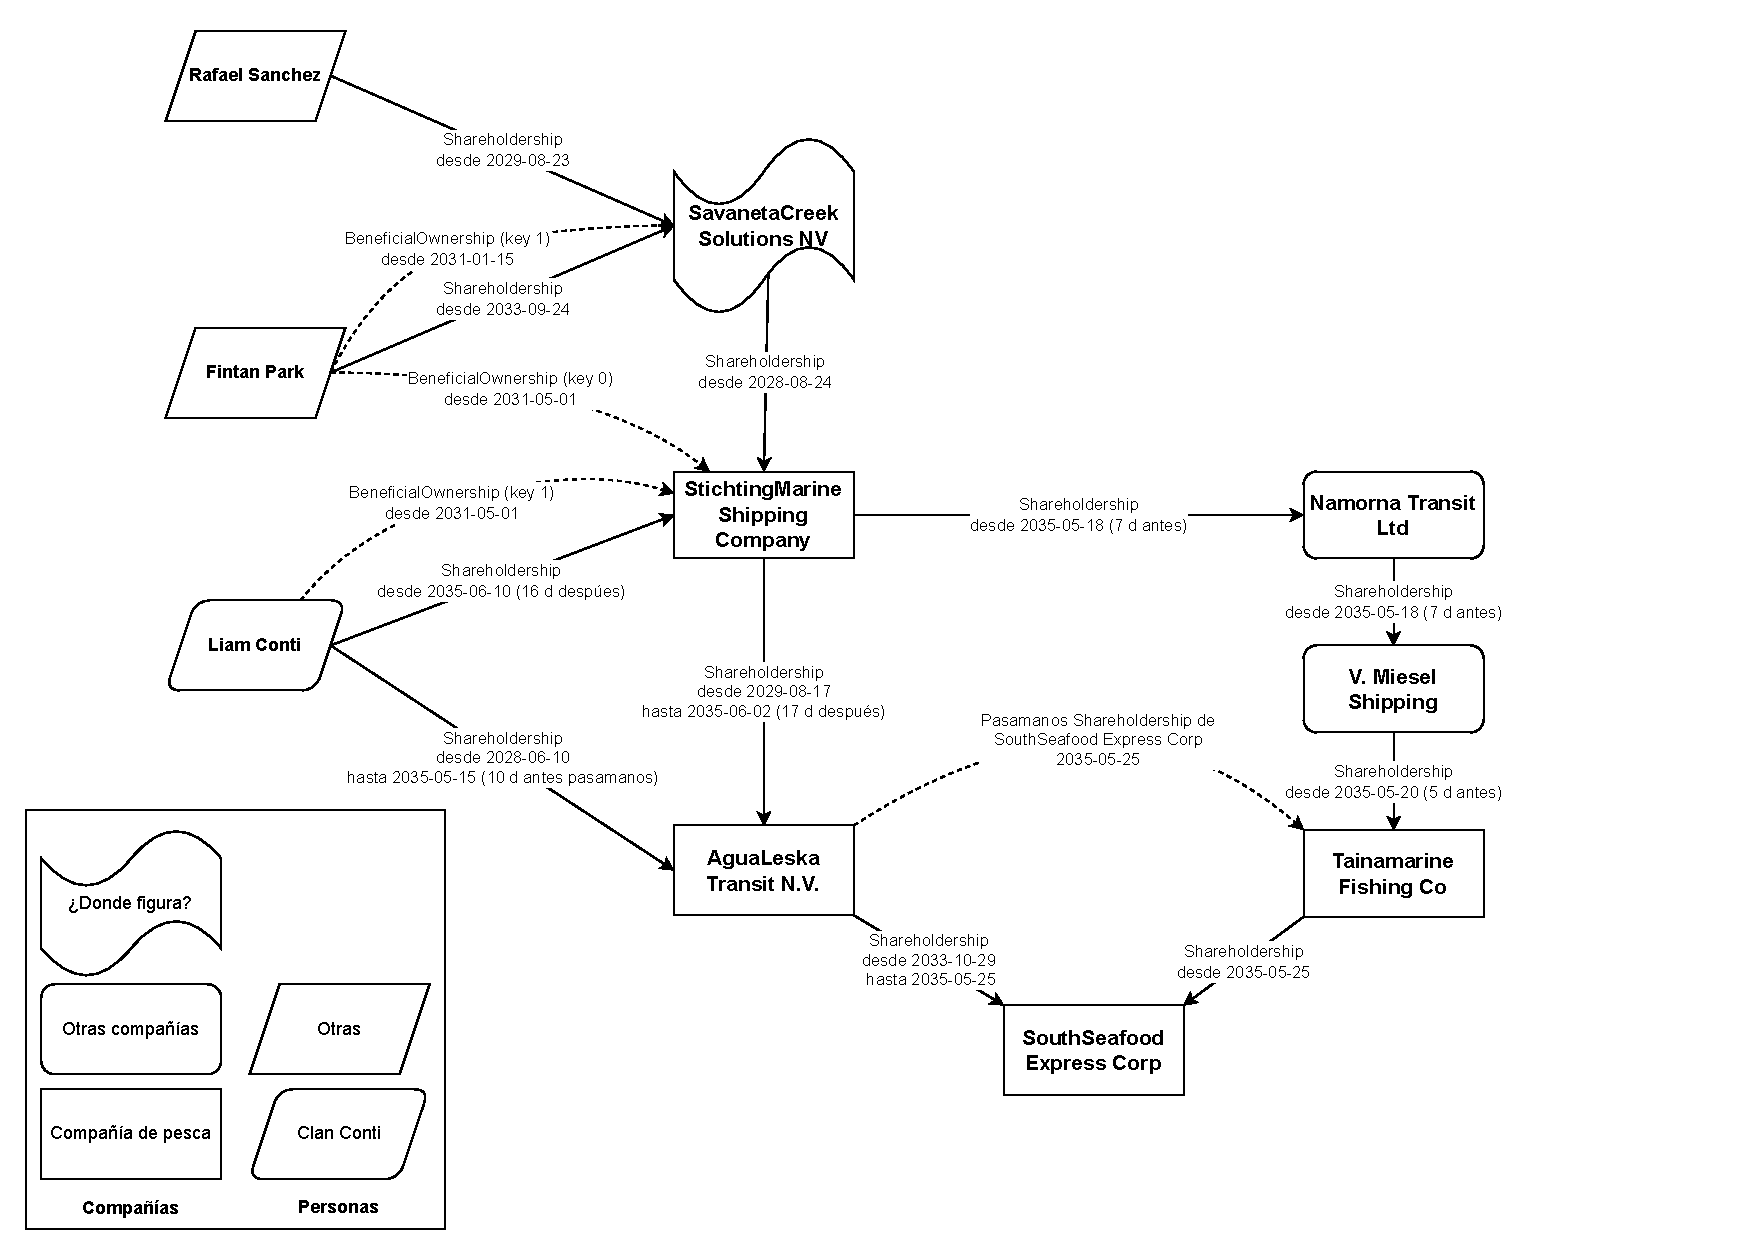
\includegraphics[width=\textwidth]{SouthSeafood.drawio.pdf}
	\caption{Red de relaciones de tenencia de acciones (shareholdership) y  beneficiario o dueño real (beneficial ownership) partiendo de \emph{SouthSeafood Express Corp} }
	\label{fig:drawio}
\end{figure}

La visualización que agrega a las relaciones de pertenencia aquella de otra índole antes (ver figura \ref{fig:antes} ) o después de esa fecha (figura \ref{fig:después}) no muestra otro cambio apreciable en torno a la misma que en la figura \ref{fig:drawio}.
Se aprecia que la red es orientada, notandose que las puntas de las flechas indican el vértice objetivo de cada arista, cuyo color indica en apartado de la base de datos.

\break

% \subsection{Venta de acciones de \emph{SouthSeafood Express Corp}}
% Es claro como 

\begin{figure}[!ht]
	\centering
	\begin{subfigure}[b]{\textwidth}
		\centering
		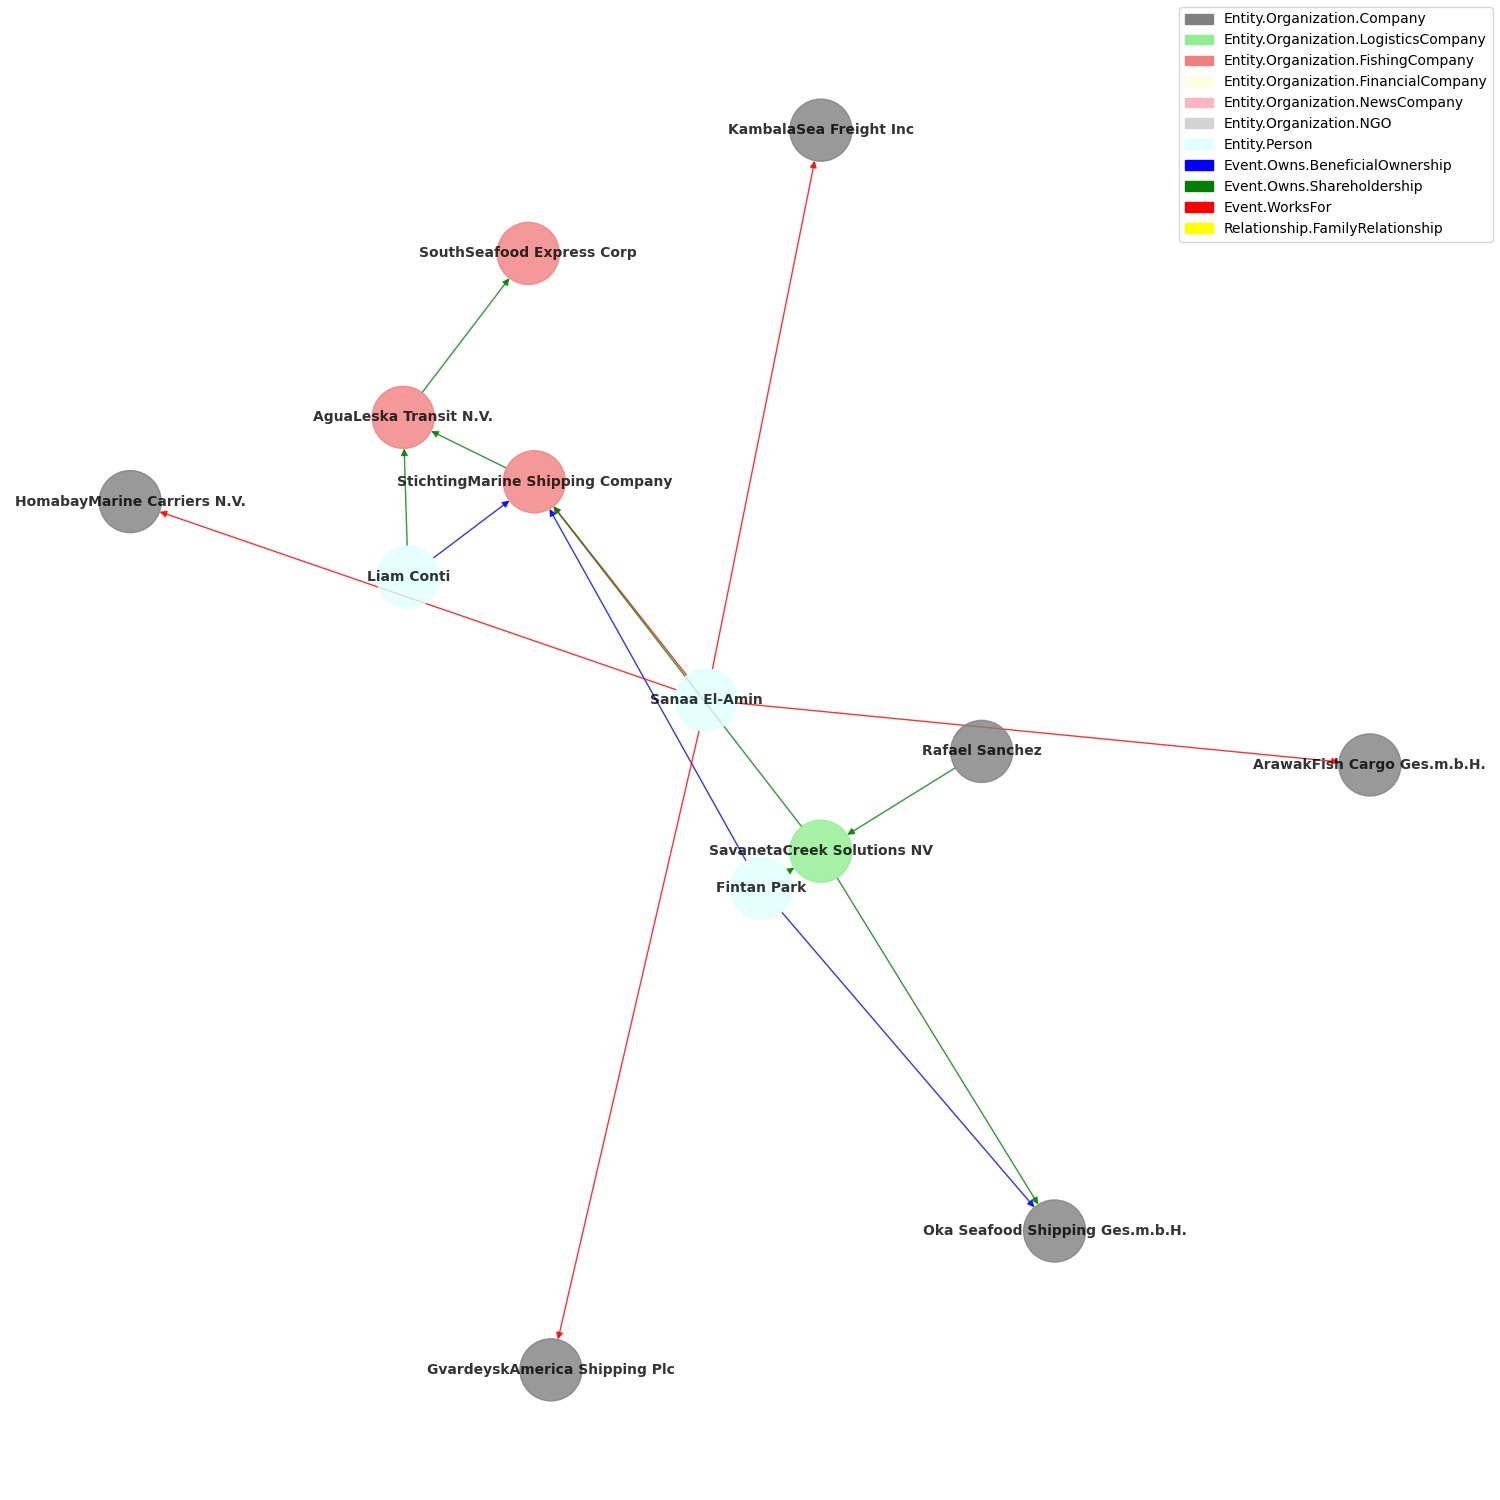
\includegraphics[width=0.6\textwidth]{eins}
		\caption{Al 2025-01-01}
		\label{fig:antes}
	\end{subfigure}
	\begin{subfigure}[b]{\textwidth}
		\centering
		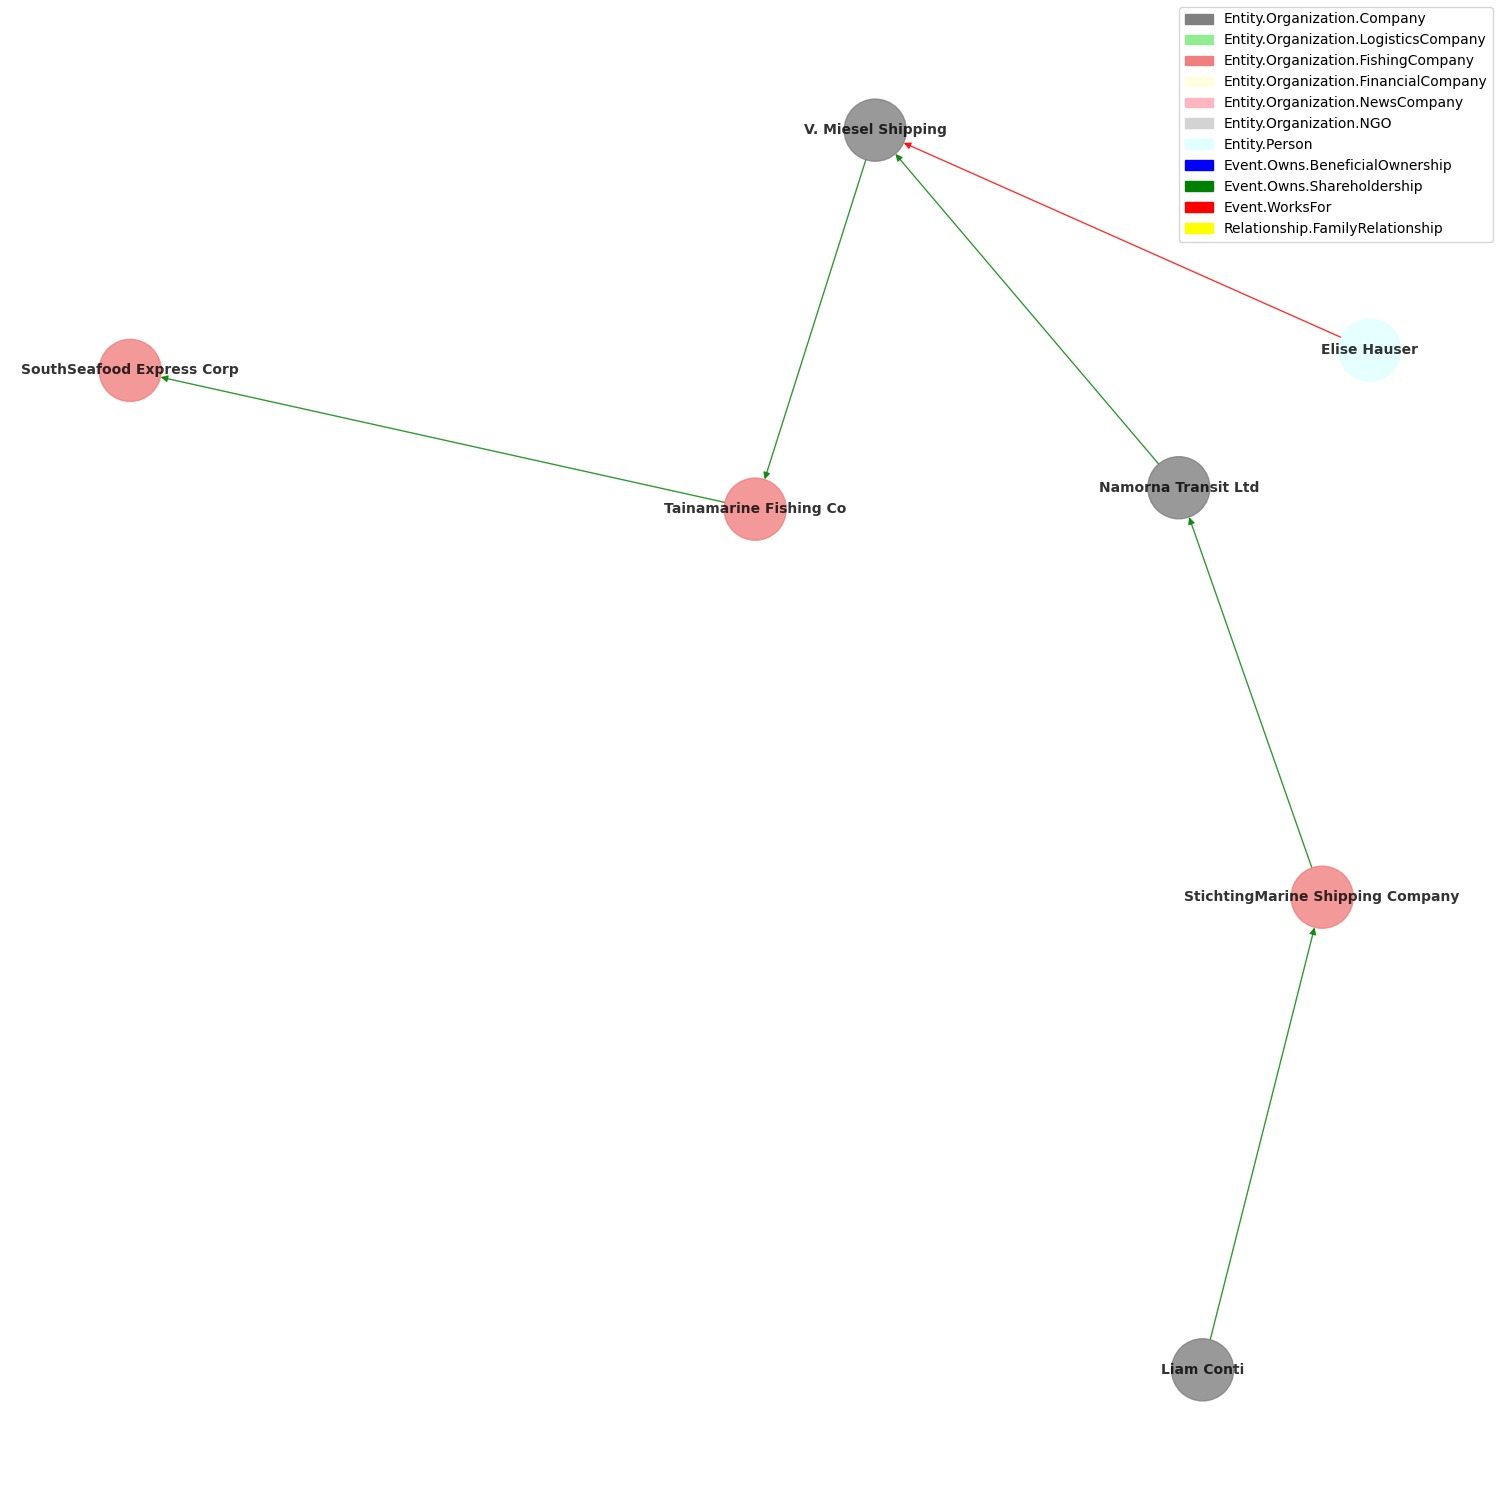
\includegraphics[width=0.6\textwidth]{zwei}
		\caption{Hacía fines de 2025}
		\label{fig:después}
	\end{subfigure}
	\caption{
		Algunas relaciones seleccionados partiendo desde \emph{SouthSeafood Express Corp} en 2025-01-01 y hacía fin de ese año.		
		}
	% \caption{Ahi van dos graficos generados, no fue tan facil como imagine, al final tuve que filtrar por el start_date, pero si tomaba la fecha 25/5 no quedaba grafo para despues asi que puse el 1/1, los anteriores a esa fecha, como era la red de SouthSea antes y los cambios durante el año, incluido varios registros sin start\_date}
	\label{fig:Networkx}
\end{figure}
\vspace{3cm}


\break

\subsection{Patrones temporales y cambios en las estructuras corporativas}

Se realizaron scatterplots con la cantidad de enlaces significativos, es decir, la cantidad de enlaces que tienen los nodos vinculados a al periodo del año 2035, contrastados con la cantidad de enlaces que tienen los mismos nodos relacionados en periodos anteriores de tiempo, utilizando la técnica de jitter para individualizar los puntos superpuestos.
En este análisis realizado para personas más activas (figura \ref{fig:personas_activas}) y empresas más activas (figura \ref{fig:empresas_activas}) durante el periodo de análisis. 

\begin{figure}[H]
    \centering
    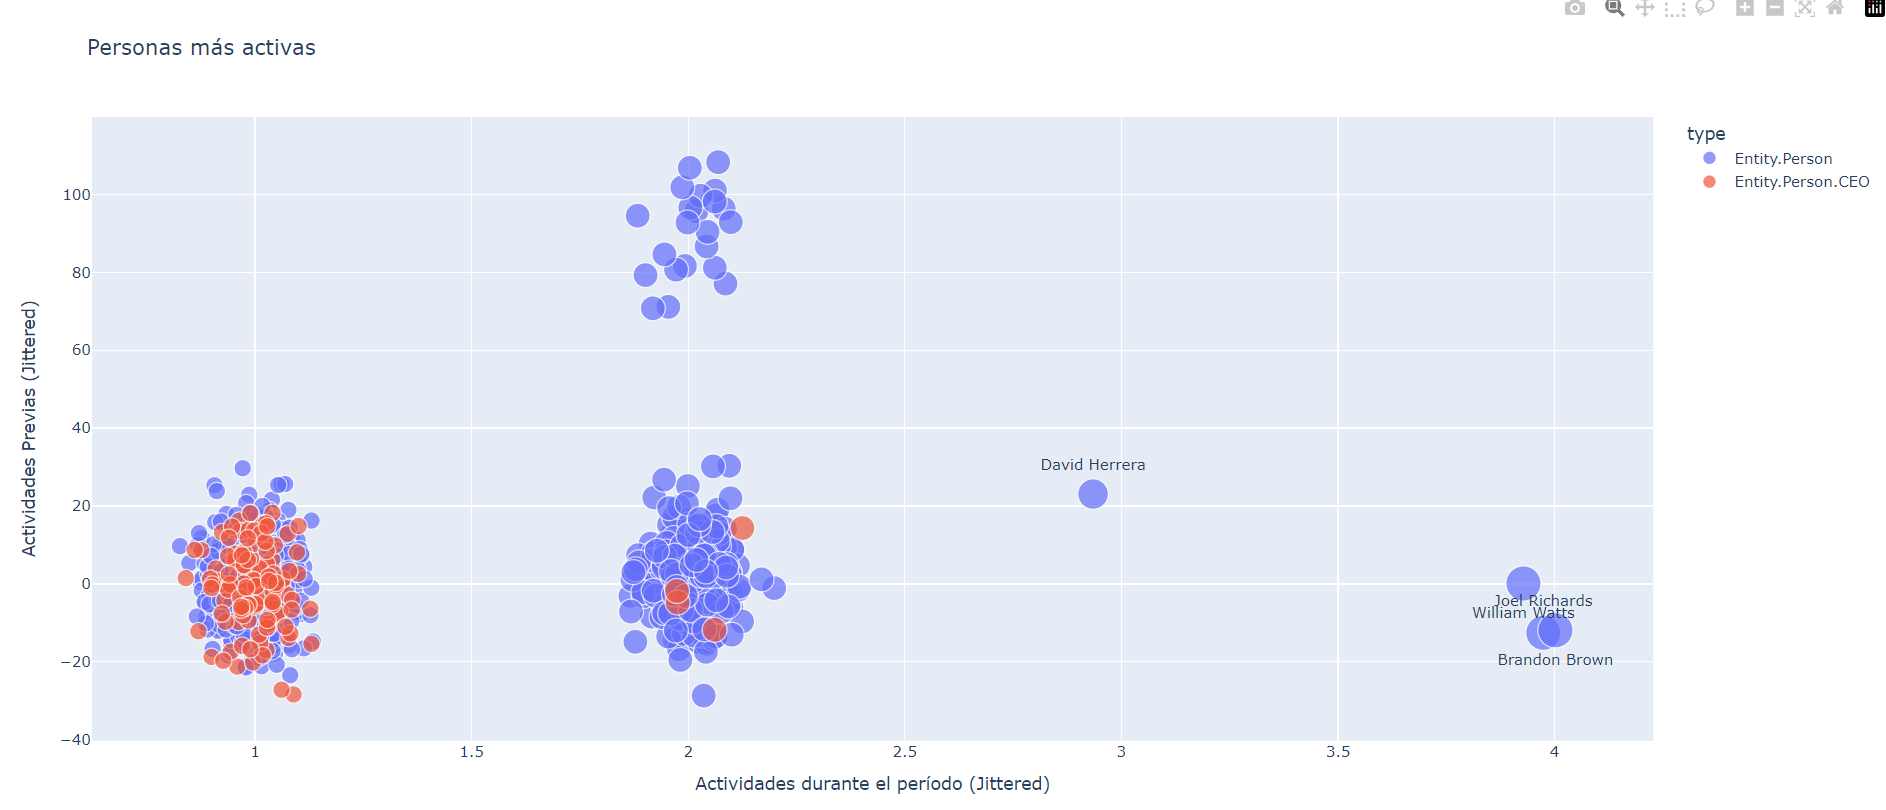
\includegraphics[width=0.7\linewidth]{graphs/ejercicio_1_2.png}
    \caption{Personas más activas. 
    La versión interactiva de esta figura es un html que puede ser descargada haciendo clik \href{https://github.com/bettachini/visualizacion/blob/main/vast2024/reporte/graphs/scatter_plot_degree_in_vs_out_period_persons_jitter.html.}{aqui}
    }
    \label{fig:personas_activas}
\end{figure}


\begin{figure}[H]
    \centering
    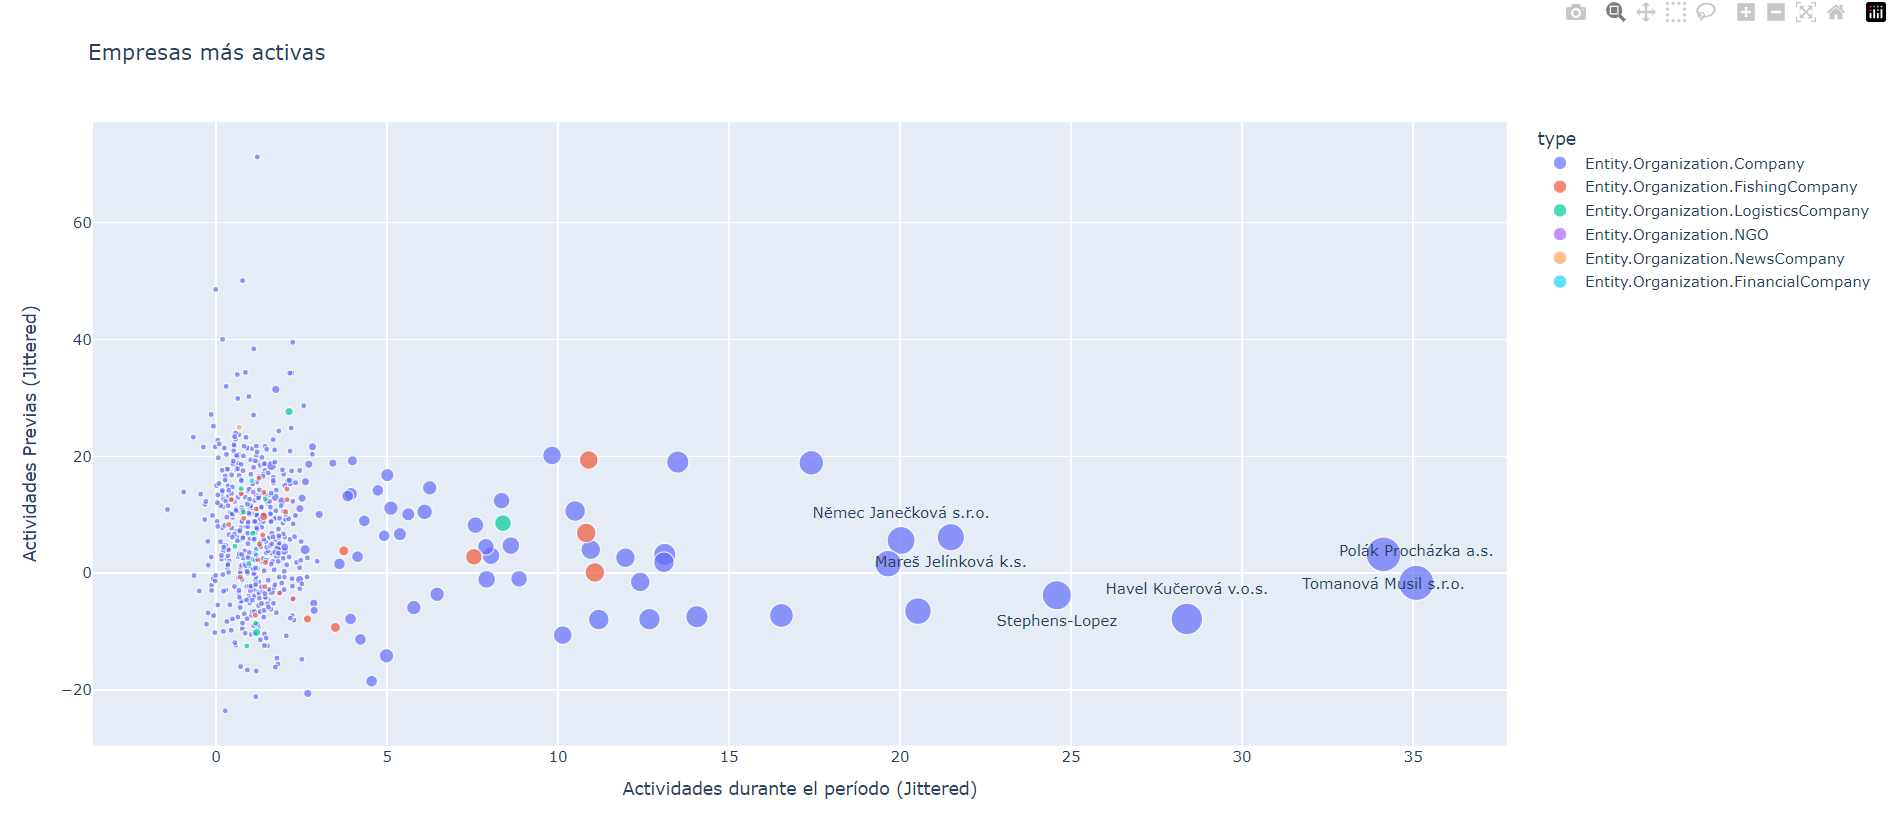
\includegraphics[width=0.9\linewidth]{graphs/ejercicio_1_1.png}
    \caption{Empresas más activas. La versión interactiva de esta figura es un html que puede ser descargada haciendo clik \href{https://github.com/bettachini/visualizacion/blob/main/vast2024/reporte/graphs/scatter_plot_degree_in_vs_out_period_companies_jitter.html}{aqui}}
    \label{fig:empresas_activas}
\end{figure}


\subsection{Estructuras corporativas}

Se buscó evidenciar patrones temporales y cambios en las estructuras corporativas a lo largo del tiempo, centrándose en la cantidad de eventos que figuran en las relaciones \emph{shareholdership}, \emph{worksfor} y \emph{beneficialownership} con diversas herramientas de visualización

Inicialmente, un gráfico de barras apiladas permitió representar la media anual de eventos de cada tipo, destacando un aumento significativo en 2034 seguido de una regresión en 2035, sugiriendo una fase de transición y posteriormente una de estabilización, como se muestra en la figura \ref{fig:medias_eventos}, en el que se aprecia en el transcurri del tiempo la media anual de eventos  de shareholdership, worksfor y beneficialownership.

\begin{figure}[H]
  \centering
  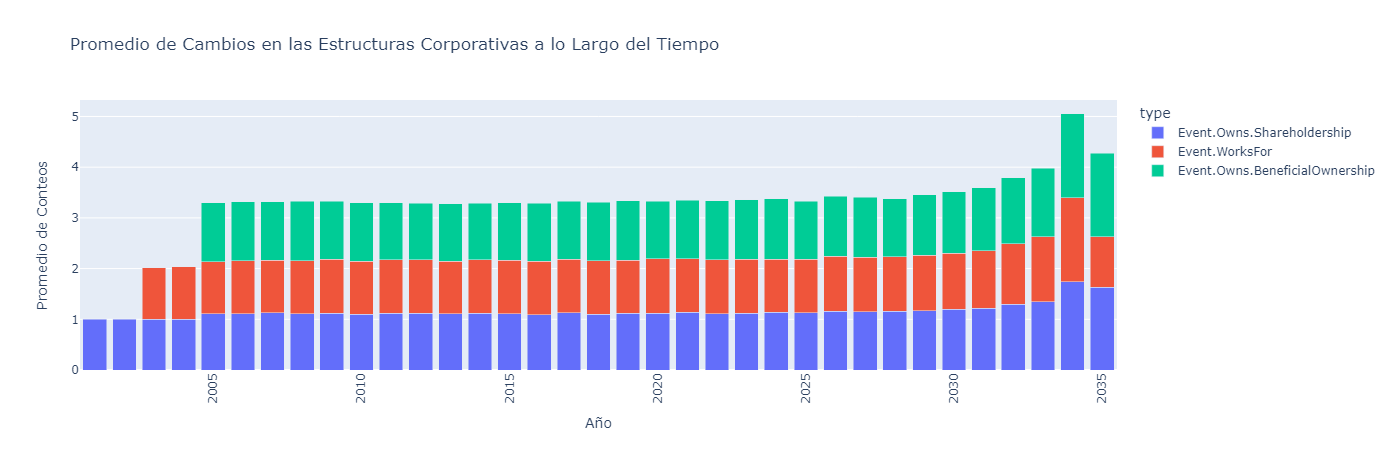
\includegraphics[width=0.7\linewidth]{graphs/promedio_cambio_estructuras.png}
  \caption{Media anual de eventos de shareholdership, worksfor y beneficialownership.}
  \label{fig:medias_eventos}
\end{figure}

La media anual de eventos entre 2005 y 2035 de beneficialownership muestra incremento marcado en los úlimos años con un pico en 2034, como se aprecia en la figura \ref{fig:beneficial_ownership_2005_2035}.
Algo similar muestra la figura \ref{fig:sharedholdership_top_anio} para shareholdership con un incremento hasta el último año de registro.

\begin{figure}[H]
  \centering
  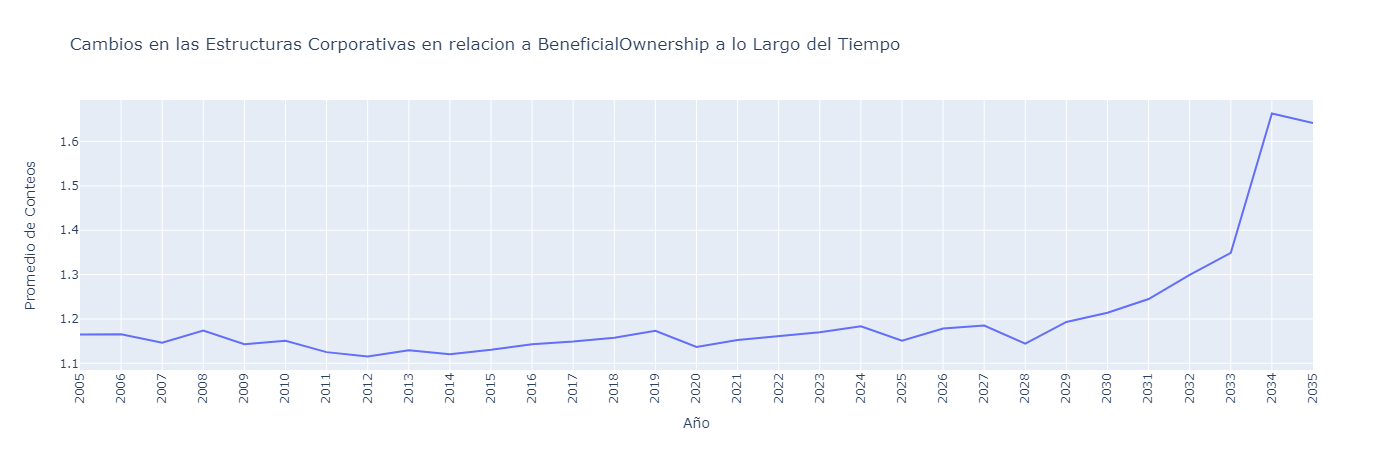
\includegraphics[width=0.7\linewidth]{graphs/promedio_cambio_beneficialOwnership.png}
  \caption{Media anual de eventos de beneficialownership de 2005 a 2035.}
  \label{fig:beneficial_ownership_2005_2035}
\end{figure}

\begin{figure}[H]
  \centering
  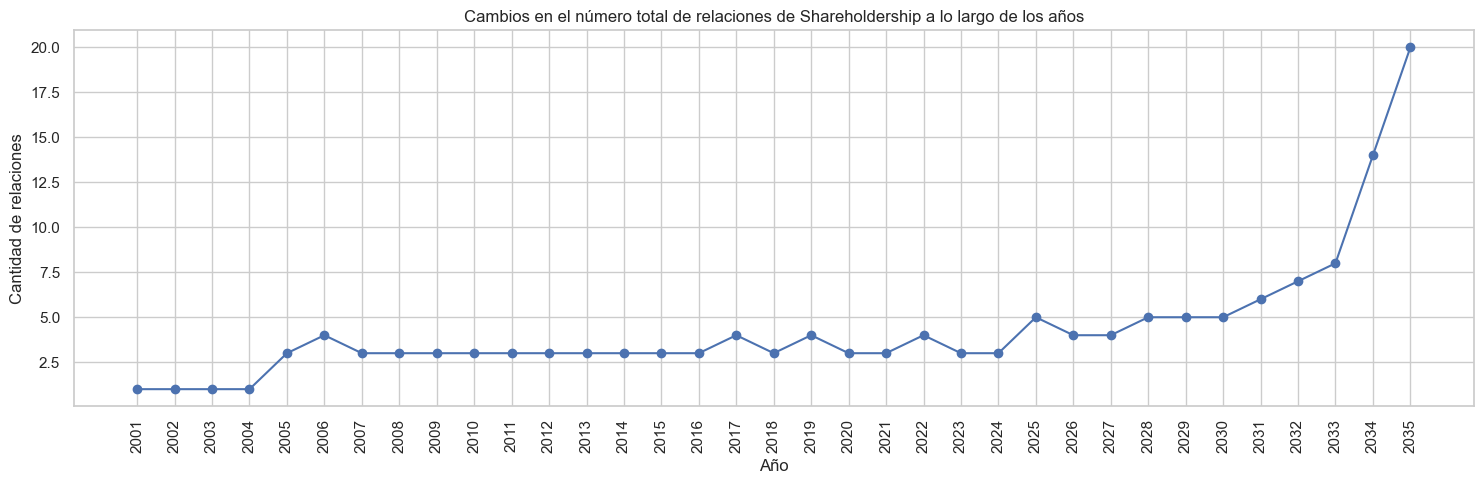
\includegraphics[width=0.7\linewidth]{graphs/dispersion_sharedholdership_top_anio_v2.png}
  \caption{Media anual de eventos de beneficialownership de 2001 a 2035.}
  \label{fig:sharedholdership_top_anio}
\end{figure}

Para identificar las empresas más prominentes en cada año según el número de eventos, se utilizó un gráfico de dispersión. Este gráfico proporciona una visualización clara de las entidades más activas a lo largo del período estudiado, con las empresas líderes debidamente identificadas y etiquetadas para facilitar la interpretación, como se ve en la figura \ref{fig:empresas_beneficial_ownership}.

\begin{figure}[H]
  \centering
  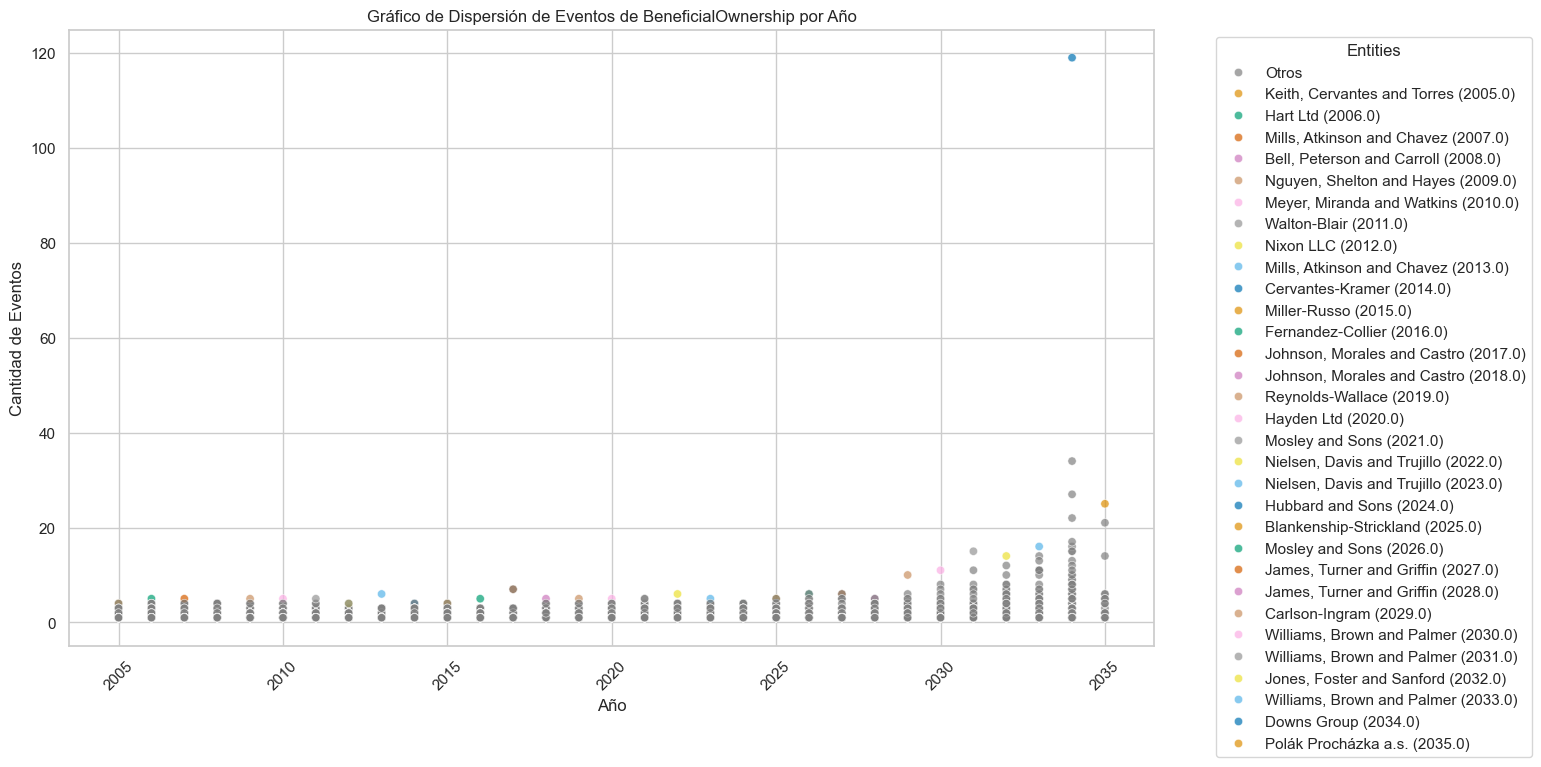
\includegraphics[width=0.7\linewidth]{graphs/dispersion_beneficialownership_top_anio.png}
  \caption{Empresas con el mayor número de eventos por año.}
  \label{fig:empresas_beneficial_ownership}
\end{figure}

Tomando en cosideración la empresa con el mayor volumen de operaciones, Downsgroup, se identificó su asociación con dos tipos distintos de entidades de beneficialownership: entity.person y entity.person.ceo. EL gráfico de barras que se muestra en la figura \ref{fig:downsgroup_ownership}, detalla la distribución de estas entidades a lo largo de los años, mostrando la predominancia de cada tipo.

\begin{figure}[H]
  \centering
  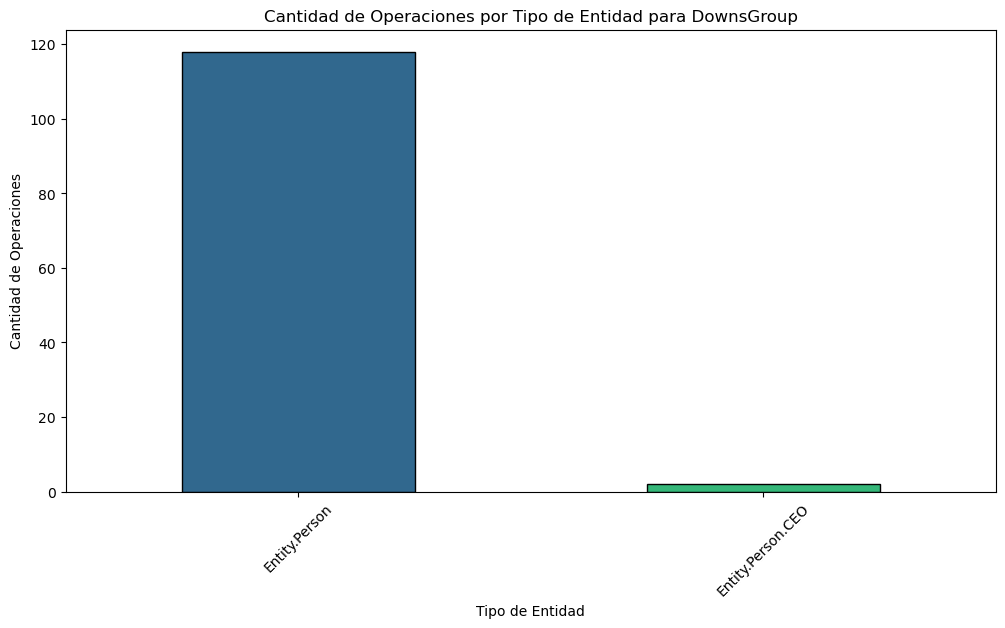
\includegraphics[width=0.7\linewidth]{graphs/distribuicion_beneficialownership_dowsgropup.png}
  \caption{Distribución de entity.person y entity.person.ceo asociadas a Downsgroup a lo largo del tiempo.}
  \label{fig:downsgroup_ownership}
\end{figure}

Finalmente, se destacaron individuos asociados al tipo entity.person.ceo con el menor número de eventos, revelando variaciones significativas en la actividad entre los participantes en este papel específico, como se presenta en la tabla de la figura \ref{fig:person_ceo_ownership}.

\begin{figure}[H]
  \centering
  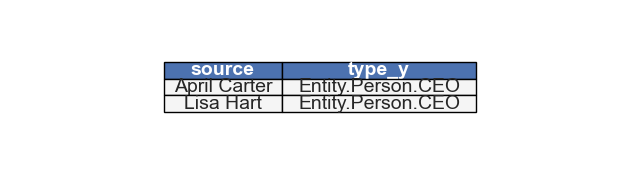
\includegraphics[width=0.7\linewidth]{graphs/person_ceo_ownership_downs.png}
  \caption{Tabla tipos de beneficialownership de DownsGroup}
  \label{fig:person_ceo_ownership}
\end{figure}

\break


Se emplearon métodos de visualización para explorar eventos de shareholdership utilizando un gráfico de líneas que muestra el aumento en 2034 en este tipo de eventos, similar al análisis de beneficialownership previamente descrito, aperciabnle en las figuras \ref{fig:shareholdership_2001_2035} y \ref{fig:shareholdership_top_anio_v2}.

\begin{figure}[H]
  \centering
  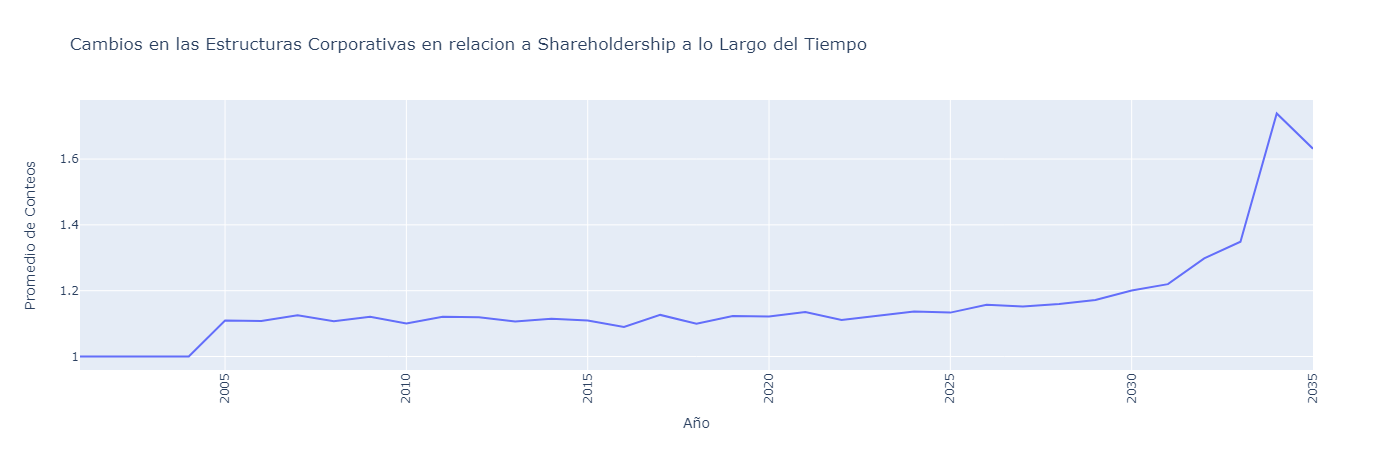
\includegraphics[width=0.7\linewidth]{graphs/promedio_cambio_shareholdership.png}
  \caption{Evolución anual de eventos de shareholdership}
  \label{fig:shareholdership_2001_2035}
\end{figure}

\begin{figure}[H]
  \centering
  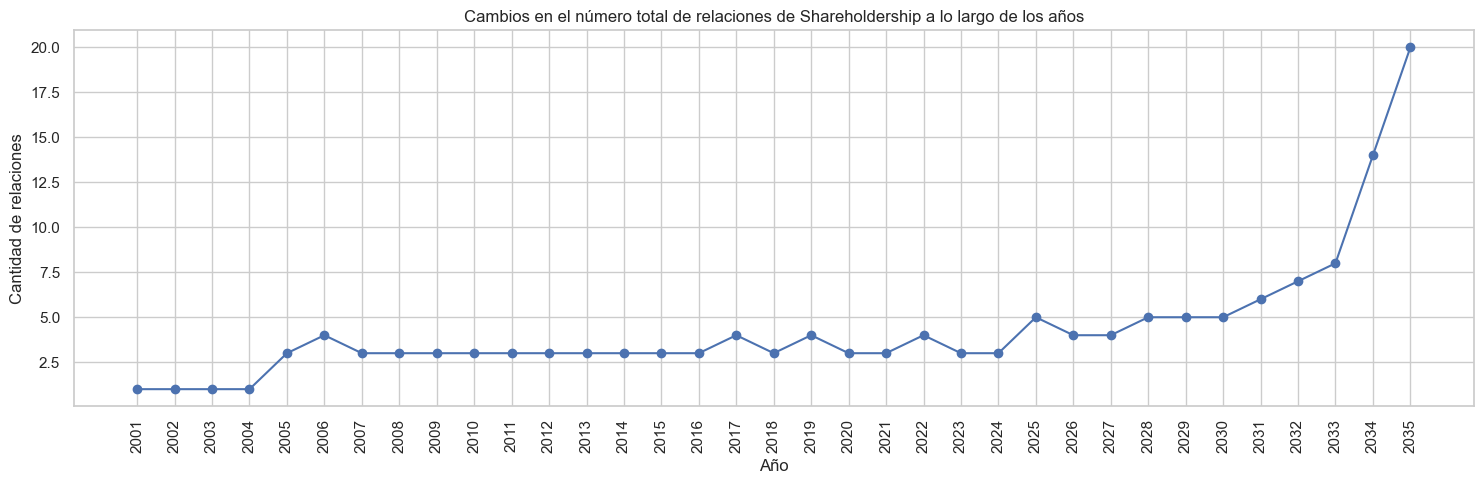
\includegraphics[width=0.7\linewidth]{graphs/dispersion_sharedholdership_top_anio_v2.png}
  \caption{Empresas con el mayor número de eventos de shareholdership por año.}
  \label{fig:shareholdership_top_anio_v2}
\end{figure}

En las figuras \ref{fig:shareholdership_empresas} y \ref{fig:empresas_numero_shareholders} se pueden identificar las empresas más destacadas en cada año por eventos de shareholdership y la cantidad de accionistas por cada empresa.

\begin{figure}[H]
  \centering
  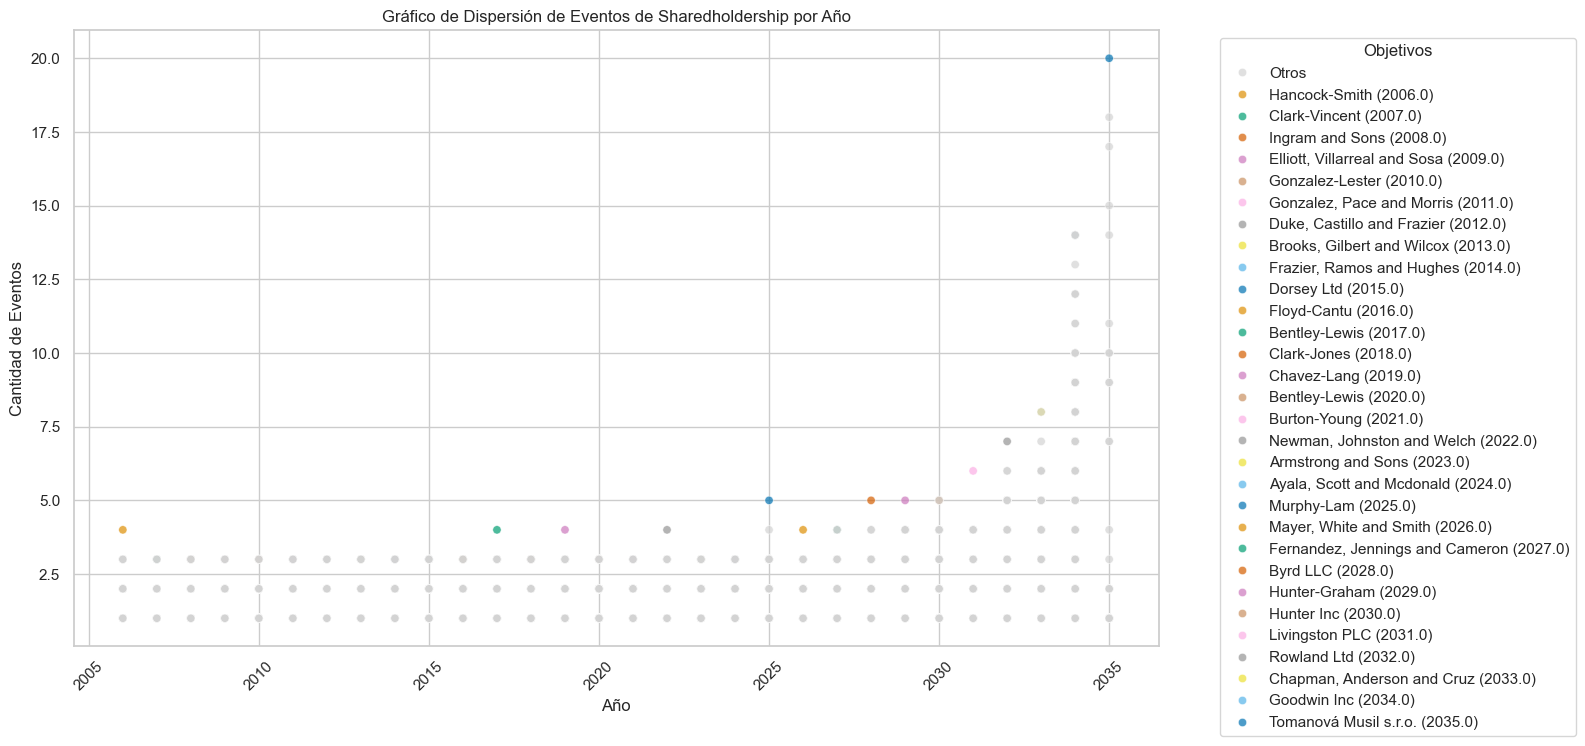
\includegraphics[width=0.7\linewidth]{graphs/dispersion_sharedholdership_top_anio.png}
  \caption{Empresas con el mayor número de eventos de shareholdership en cada año.}
  \label{fig:shareholdership_empresas}
\end{figure}

\begin{figure}[H]
  \centering
  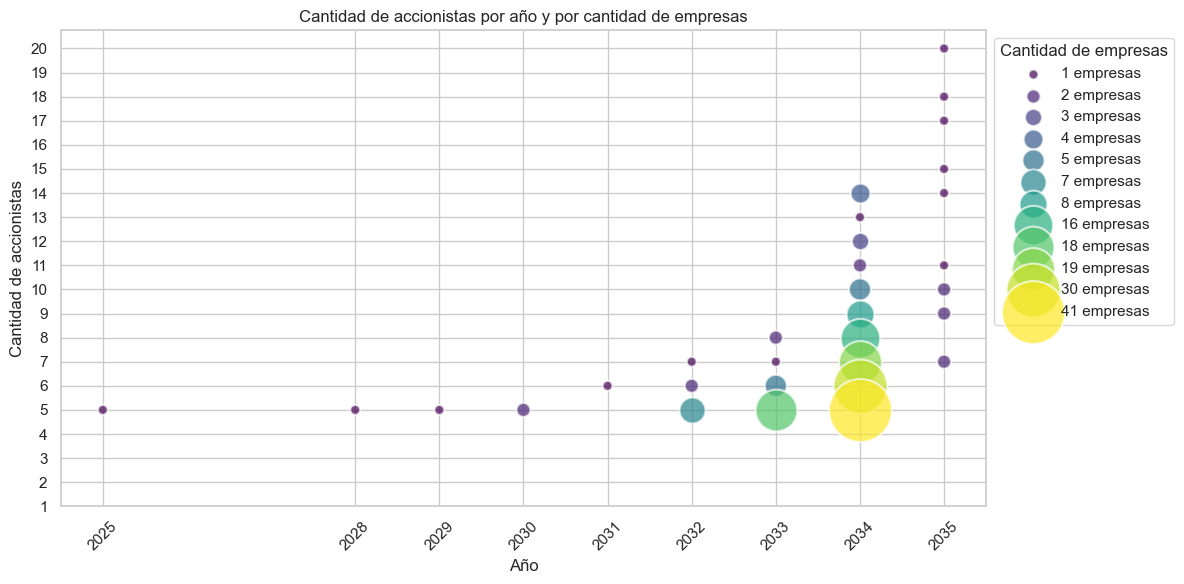
\includegraphics[width=0.7\linewidth]{graphs/cant_empresas_con_numero_shareholders_anio.png}
  \caption{Cantidad de accionistas por empresa y fecha.}
  \label{fig:empresas_numero_shareholders}
\end{figure}

Posteriormente, se creó un gráfico de barras figura \ref{fig:principales_objetivos_shareholdership} que muestra
Para visualizar las empresas con más eventos de shareholdership y el año en que cada una alcanzó su mayor cantidad de eventos se utiliza un gráfico de barras como se aprecia en la figura \ref{fig:principales_objetivos_shareholdership}. La empresa con más eventos es Tomanová Musil s.r.o., para la cual en la tabla, de la figura \ref{fig:shareholdership_tomanova}, se identifican sus shareholdership en 2035.

\begin{figure}[H]
  \centering
  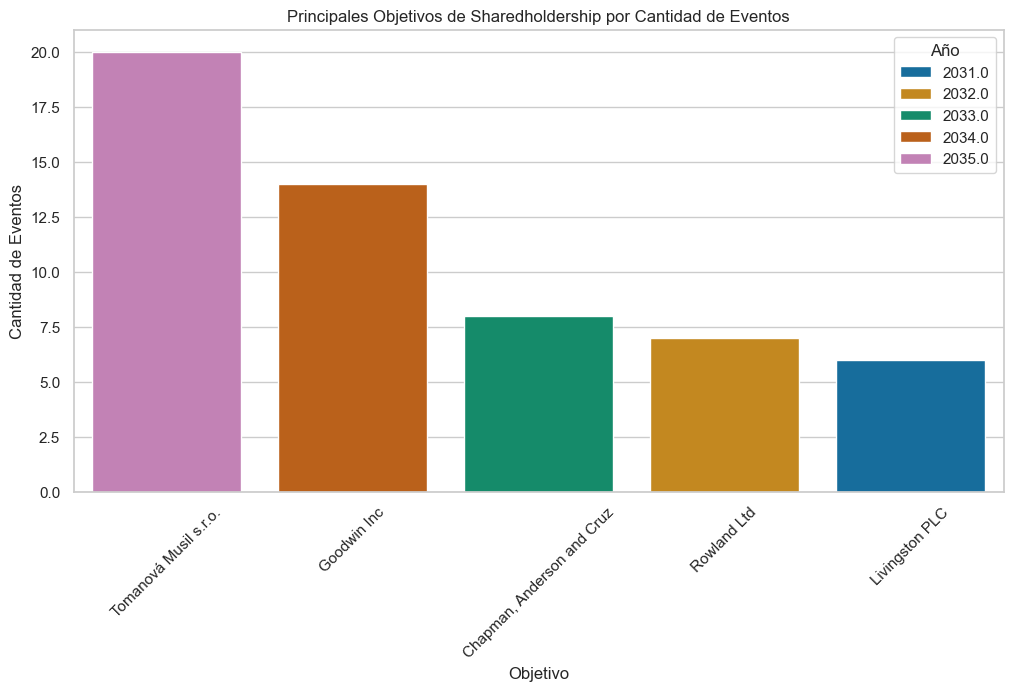
\includegraphics[width=0.7\linewidth]{graphs/principales_objetivos_sharedholdership.png}
  \caption{Empresas con más eventos de shareholdership y el año de mayor actividad.}
  \label{fig:principales_objetivos_shareholdership}
\end{figure}

\begin{figure}[H]
  \centering
  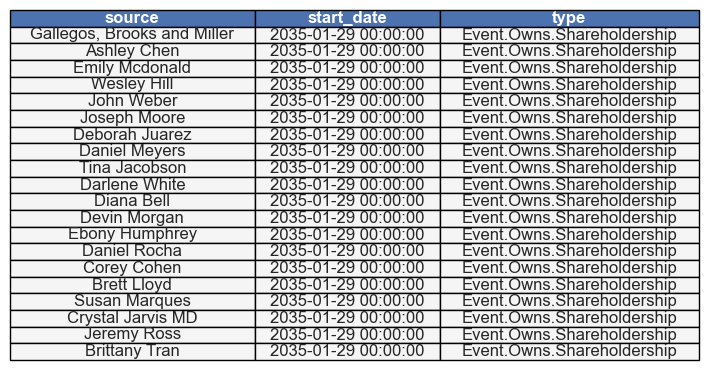
\includegraphics[width=0.7\linewidth]{graphs/tabla_sharedholdership_tomanova_20235.png}
  \caption{ShareholderShip Tomanová Musil s.r.o.}
  \label{fig:shareholdership_tomanova}
\end{figure}

Para profundizar en el análisis, se examinaron los tipos de entity que se convirtieron en shareholdership en 2035 para Tomanová Musil s.r.o figura \ref{fig:distribuicion_shareholdership_tomanova}. Se encontró que de un total de 20 shareholdership, solo uno fue del tipo Entity.Organization.Company, mientras que los otros 19 fueron del tipo Entity.Person. La tabla que muestra esta única compañía, se aprecia en la figura \ref{fig:entity_company_shareholder_tomanova}.

\begin{figure}[H]
  \centering
  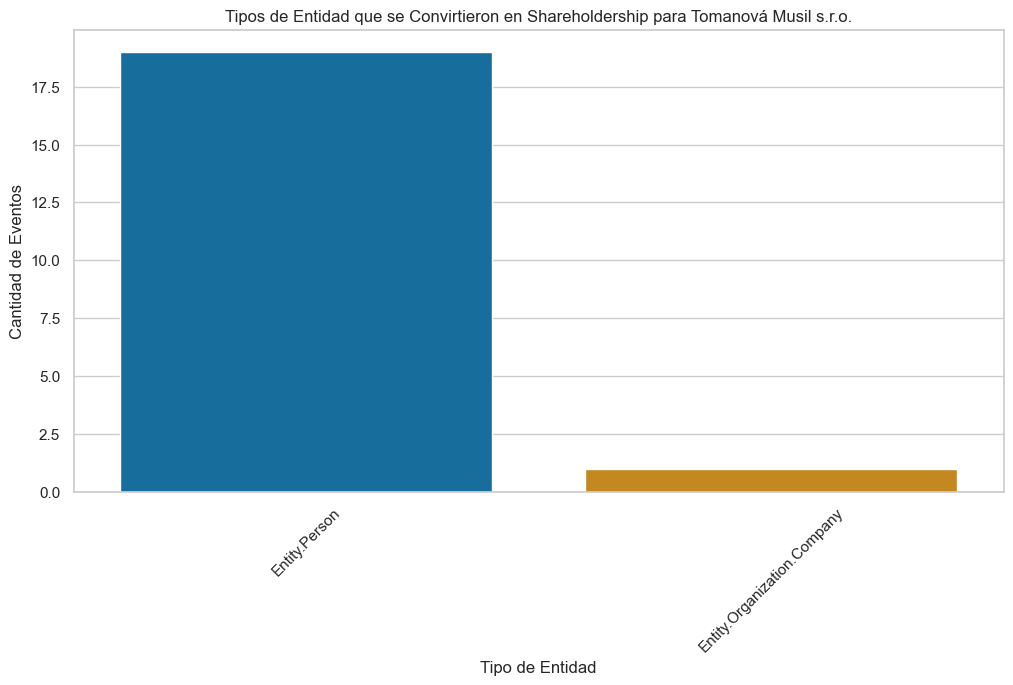
\includegraphics[width=0.7\linewidth]{graphs/distribuicion_shareholdership_tomanova.png}
  \caption{Shareholdership del tipo Entity.Organization.Company para Tomanová Musil s.r.o. en 2035.}
  \label{fig:distribuicion_shareholdership_tomanova}
\end{figure}

\begin{figure}[H]
  \centering
  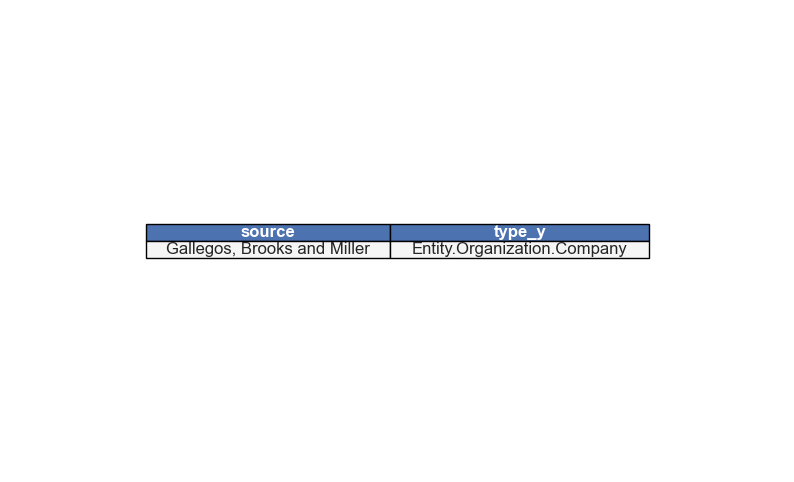
\includegraphics[width=0.7\linewidth]{graphs/entity_company_shareholder_tomanova.png}
  \caption{Shareholdership del tipo Entity.Organization.Company para Tomanová Musil s.r.o. en 2035.}
  \label{fig:entity_company_shareholder_tomanova}
\end{figure}


Observando los eventos de worksfor, la cantidad de contrataciones por año y como este número cambia. Para revisar esto, se crea un gráfico de barras para mostrar el aumento de la media de contrataciones en 2034, similar a los patrones observados en otros tipos de eventos, como se muestra en las figuras \ref{fig:contrataciones_2001_2035} y \ref{fig:contrataciones_2001_2035_v2}.

\begin{figure}[H]
  \centering
  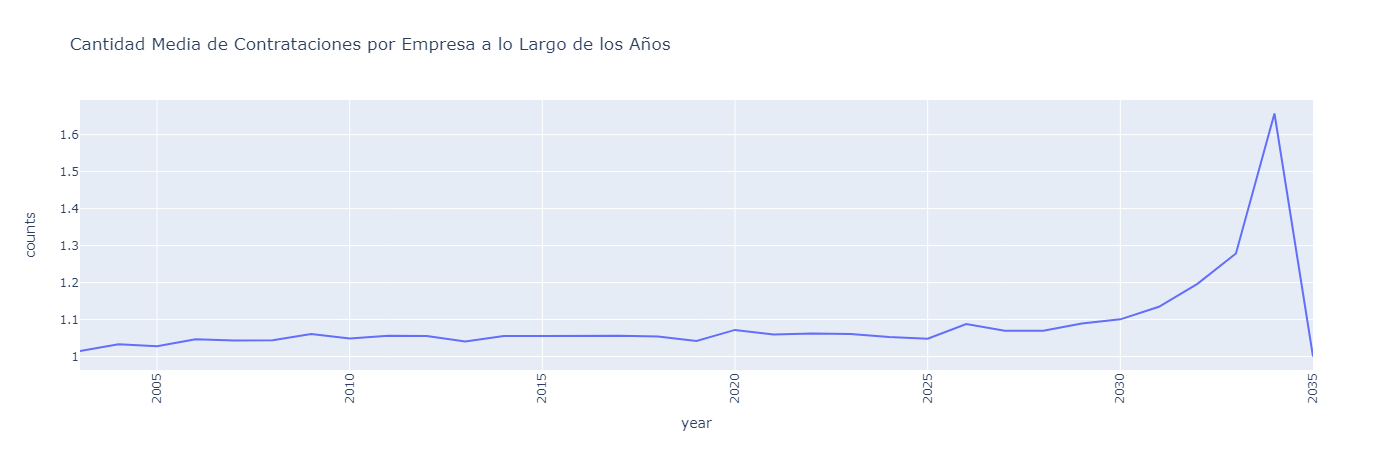
\includegraphics[width=0.7\linewidth]{graphs/promedio_cambio_contrataciones.png}
  \caption{Media anual de contrataciones (worksfor) por empresa, destacando el aumento en 2034.}
  \label{fig:contrataciones_2001_2035}
\end{figure}

\begin{figure}[H]
  \centering
  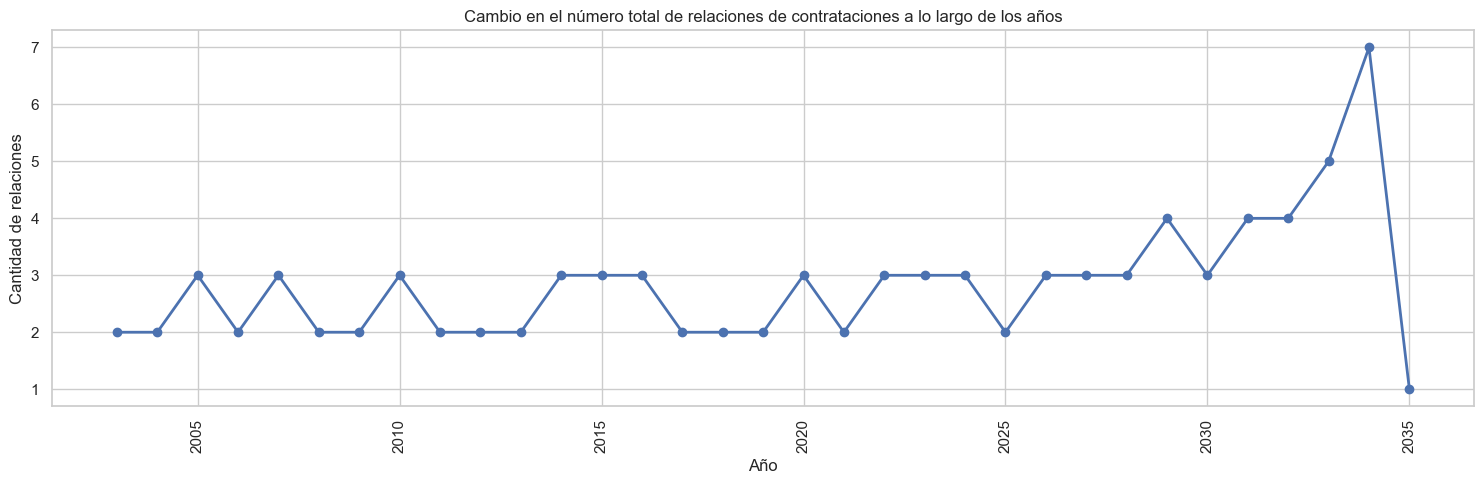
\includegraphics[width=0.7\linewidth]{graphs/promedio_cambio_contrataciones_v2.png}
  \caption{Media anual de contrataciones (worksfor) por empresa, destacando el aumento en 2034.}
  \label{fig:contrataciones_2001_2035_v2}
\end{figure}

Se utilizó un gráfico de dispersión para mostrar la cantidad de contrataciones que cada empresa realizó por año, observable en la figura \ref{fig:dispersion_contrataciones}. De este resultado se destacaron las empresas principales de cada año y cuando existe más de una empresa líder y fueron agrupadas bajo la leyenda ``Otros".

\begin{figure}[H]
  \centering
  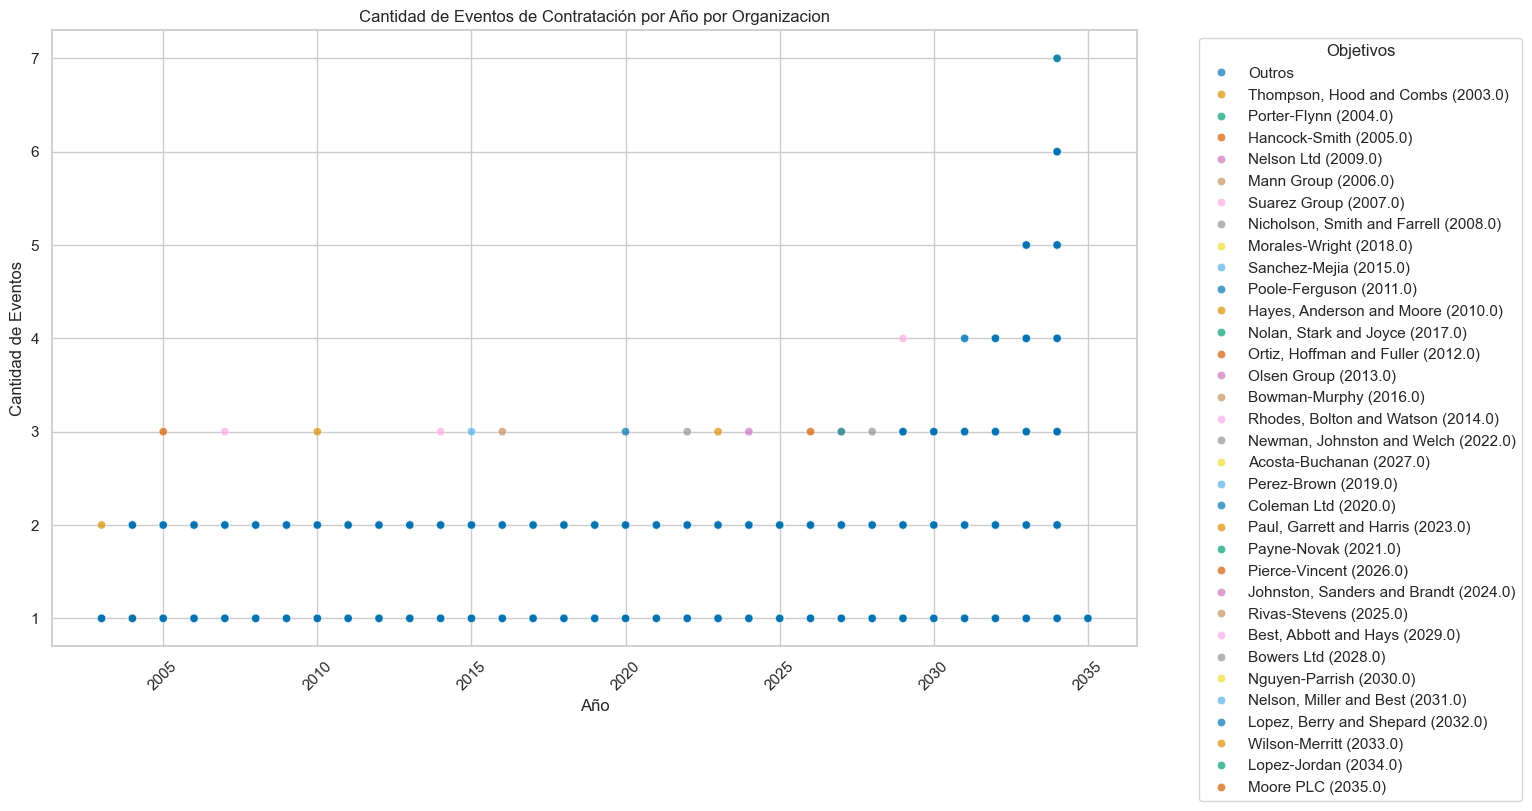
\includegraphics[width=0.7\linewidth]{graphs/dispersion_contrataciones_top_anio.png}
  \caption{Empresas con más contrataciones (worksfor) por año, destacando la empresa líder de cada año.}
  \label{fig:dispersion_contrataciones}
\end{figure}

Para un análisis más detallado, se filtraron y listaron las 5 empresas con más contrataciones y el año correspondiente de cada contratación en una tabla, como se muestra en la figura \ref{fig:top_contrataciones}.

\begin{figure}[H]
  \centering
  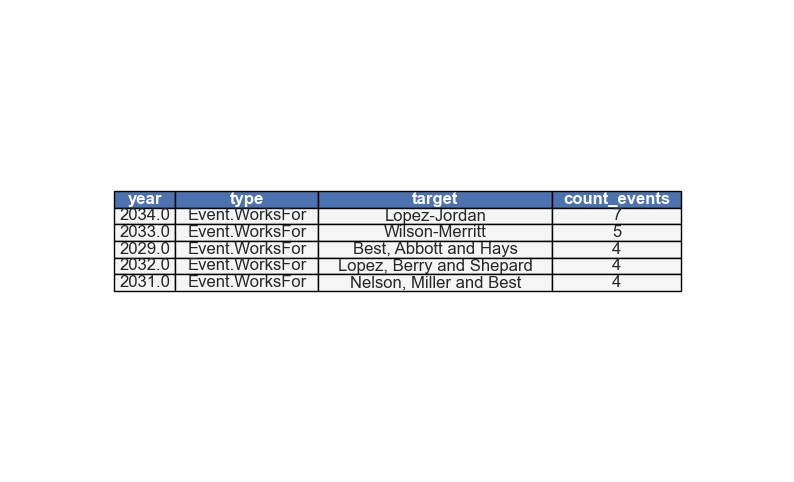
\includegraphics[width=0.7\linewidth]{graphs/tabla_top_contratasciones_anio.png}
  \caption{Empresas con más contrataciones (worksfor) y el año de mayor actividad.}
  \label{fig:top_contrataciones}
\end{figure}

Esta aproximación visual y analítica ofrece un análisis detallado de las contrataciones por empresa a lo largo del tiempo, proporcionando perspectivas sobre las dinámicas de contratación y las empresas más activas en este aspecto.


\subsection{Transacciones típicas y atípicas}

\begin{figure}[H]
    \centering
    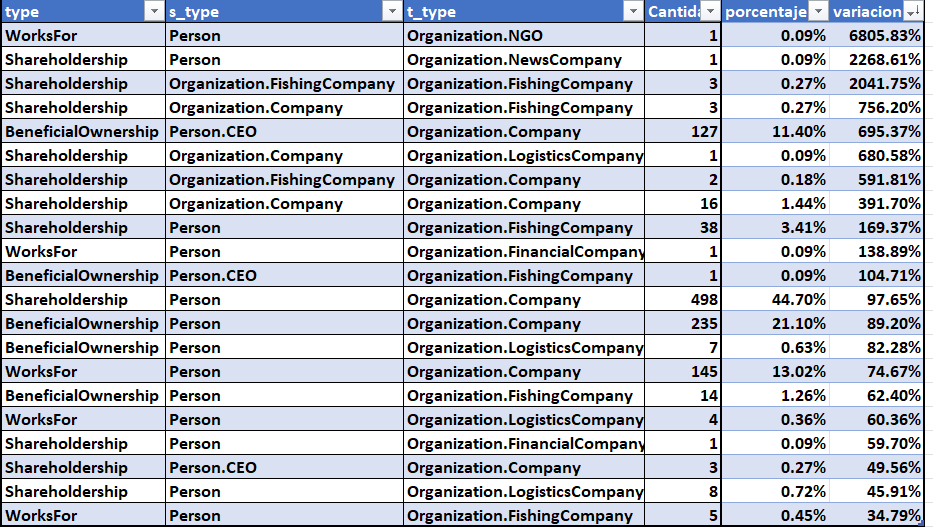
\includegraphics[width=0.7\linewidth]{graphs/ejercicio_2_0_.png}
    \caption{Resumen por tipo de transacción y entidades involucradas}
    \label{fig:enter-label3}
\end{figure}

En la Figura \ref{fig:enter-label3} se puede observar el tipo y cantidad de transacciones que se realizaron durante el año 2035 en la comunidad de Oceanus, discriminado por las entidades target y source involucradas en las mismas, también figura el porcentaje que representa la misma con respecto a la totalidad de las realizadas durante ese año y en al última columna figura la relación entre ese porcentaje y el porcentaje total que existe de ese tipo de transacción (tipo de transacción, tipo de entidad source y target) en la base de datos.

La tabla que reproduce la figura \ref{fig:enter-label4} muestra ejemplos de transacciones comerciales típicas y atípicas (por ejemplo, fusiones, adquisiciones, etc.), que pueden atender a la pregunta de si ``¿Pueden inferirse las motivaciones detrás de los cambios en su actividad?''

\begin{figure}[H]
    \centering
    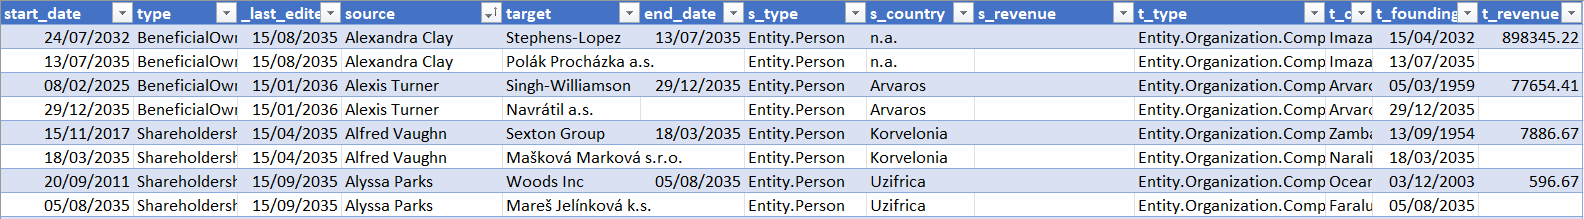
\includegraphics[width=1\linewidth]{graphs/ejercicio_2_1.png}
    \caption{Ejemplo transacciones típicas}
    \label{fig:enter-label4}
\end{figure}


\paragraph{Transacción Típica: Venta y Compra de Empresas}
Es común observar en una buena cantidad de los movimientos durante el periodo observado donde una persona vende sus acciones o la propiedad de una empresa mientras simultáneamente adquiere una nueva entidad. Este tipo de transacción puede ser motivado por diversas razones estratégicas y financieras.

Imaginemos el caso de Alexis Turner, quien recientemente vendió su participación en Singh-Williamson, una compañía establecida con una trayectoria financiera consolidada. Al mismo tiempo, Alexis adquirió Arvaros, una empresa relativamente nueva que aún no ha declarado ganancias significativas en el último año fiscal.

Esta transacción es típica en el sentido de que Alexis optó por diversificar su cartera de inversiones. Al vender en una empresa con estabilidad financiera probada como Singh-Williamson, podría asegurar ganancias acumuladas mientras transfiere sus recursos a Arvaros, una empresa que, aunque nueva en el mercado, podría tener un potencial de crecimiento considerable en el futuro.

\paragraph{Transacción Atípica: Compra de Acciones para Ocultar Propietarios}
Por otro lado, existen transacciones menos convencionales que podrían tener motivaciones menos claras. Tomemos el ejemplo reciente de SouthSeafood Express Corp, una empresa de pesca marítima que adquirió acciones significativas en AguaLeska Transit N.V. y Tainamarine Fishing Co.

\begin{figure}[H]
    \centering
    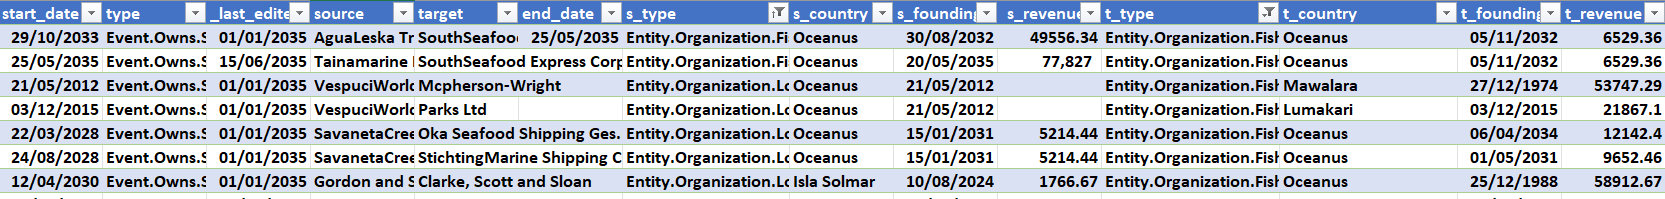
\includegraphics[width=1\linewidth]{graphs/ejercicio_2_2.png}
    \caption{Transacción atípica}
    \label{fig:enter-label5}
\end{figure}

Estas adquisiciones podrían no solo representar una expansión estratégica en el sector pesquero, sino también levantar interrogantes sobre la intención de ocultar la verdadera propiedad de SouthSeafood Express Corp. Al comprar y vender acciones entre varias entidades, especialmente cuando una de ellas es relativamente nueva como AguaLeska Transit N.V., la empresa podría estar utilizando estas transacciones para enmascarar a los verdaderos propietarios o para evadir ciertas obligaciones regulatorias.

Estos casos atípicos subrayan la importancia de una diligencia debida exhaustiva en las transacciones comerciales. Es crucial para los reguladores y partes interesadas comprender las motivaciones detrás de tales movimientos financieros para garantizar la transparencia y la integridad del mercado.

\subsection{Inferencia de importancia y ownership mediante visualización}

\paragraph{Inferencia de influencia mediante visualización}
Para abordar este problema, se generaron tres gráficos para cada medida de centralidad, mostrando cómo evolucionó cada centralidad entre 2005 y 2035 para las empresas que más experimentaron cambios en esas centralidades.

\begin{figure}[H]
  \centering
  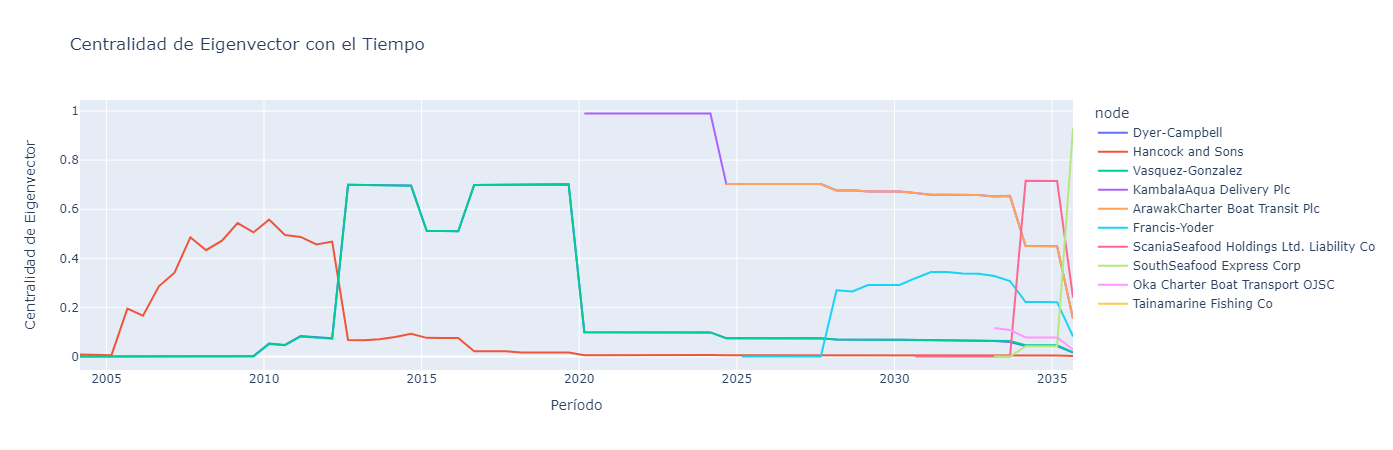
\includegraphics[width=0.7\linewidth]{graphs/eigenvector_centralidad_tiempo.png}
  \caption{Evolución de centralidad de autovector para las empresas con más cambios.}
\end{figure}

\begin{figure}[H]
  \centering
  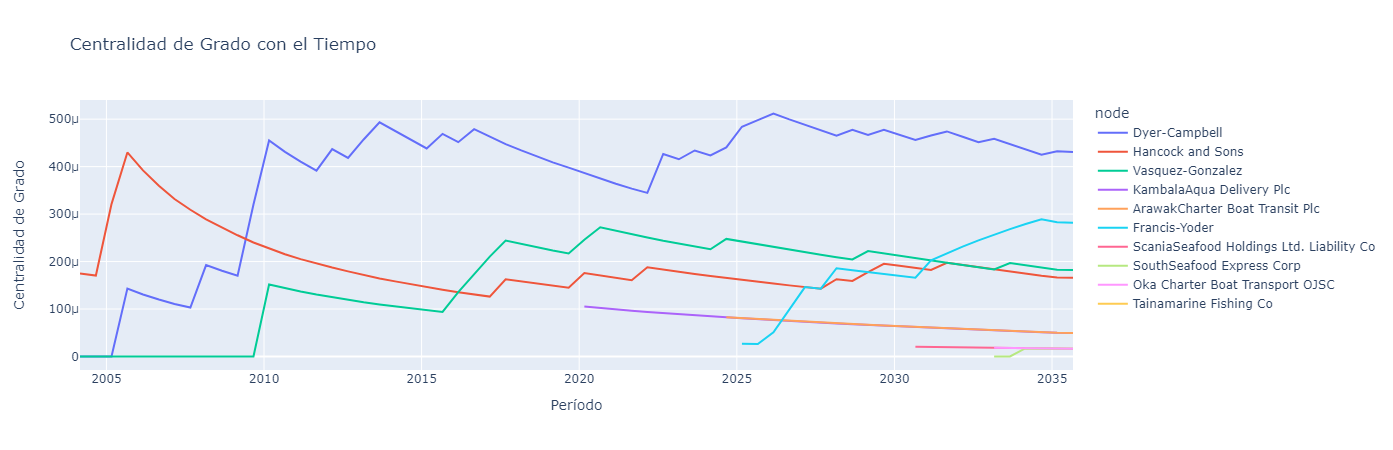
\includegraphics[width=0.7\linewidth]{graphs/grado_centralidad_tiempo.png}
  \caption{Evolución de centralidad de grado para las empresas con más cambios.}
\end{figure}

\begin{figure}[H]
  \centering
  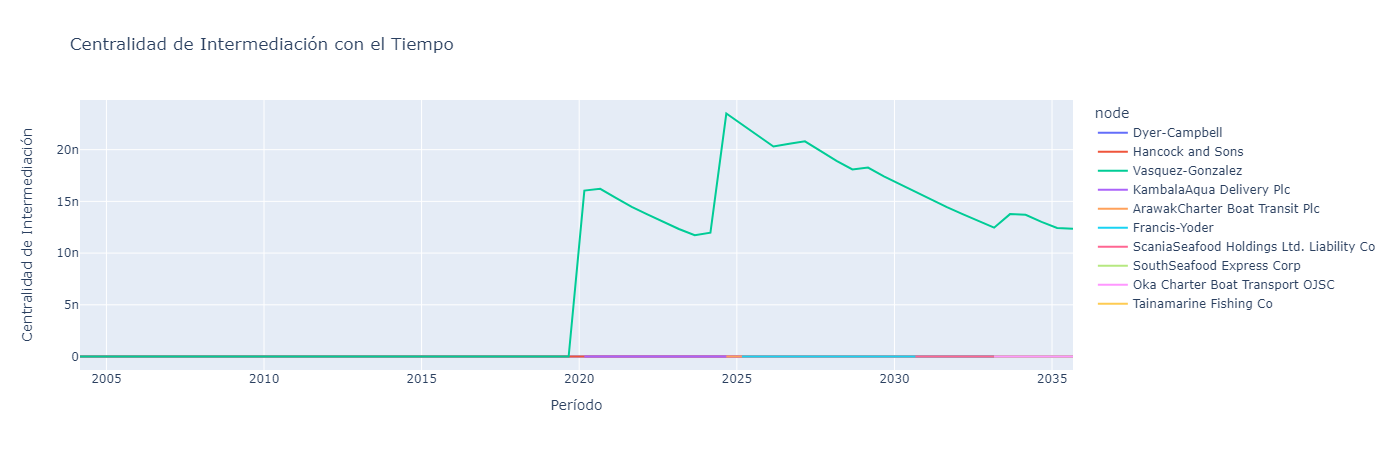
\includegraphics[width=0.7\linewidth]{graphs/between_centralidad_tiempo.png}
  \caption{Evolución de centralidad de intermediación para las empresas con más cambios.}
\end{figure}

En los gráficos siguientes mostrados en las figuras \ref{fig:cent_grado_a_VG}, \ref{fig:cent_grado_g_VG} y \ref{fig:cent_grado_i_VG}, se puede notar, que al usa el ejemplo de la empresa Vásquez-González, podemos observar que casi 20 años después de su fundación, en 2010 comenzó a tener más influencia en la red. Analizando los datos, parece que esto ocurrió debido a un cambio de propiedad a McPherson-Wright, ya que aumentó de 0.1 a 0.6 en un solo período, mostrando un crecimiento rápido. Después de un tiempo, su influencia disminuyó, la empresa fue vendida a otra persona y luego volvió a aumentar. Hasta que en 2020 comenzó a disminuir y se estabilizó con una influencia que se imagina como la normal. Incluso con una influencia baja, mantuvo grados y centralidad más estables, y se pudo inferir cosas sobre la propiedad también.

\begin{figure}[H]
  \centering
  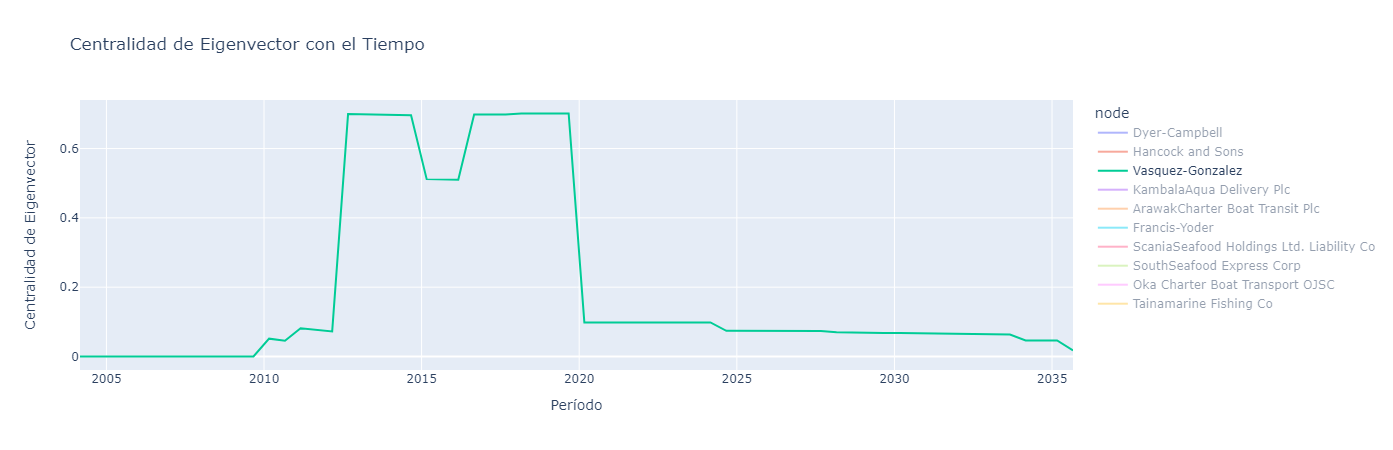
\includegraphics[width=0.7\linewidth]{graphs/eigenvector_centralidad_tiempo_vasquez.png}
  \caption{Evolución de centralidad de autovector para la empresa Vasquez-Gonzalez.}
  \label{fig:cent_grado_a_VG}
\end{figure}

\begin{figure}[H]
  \centering
  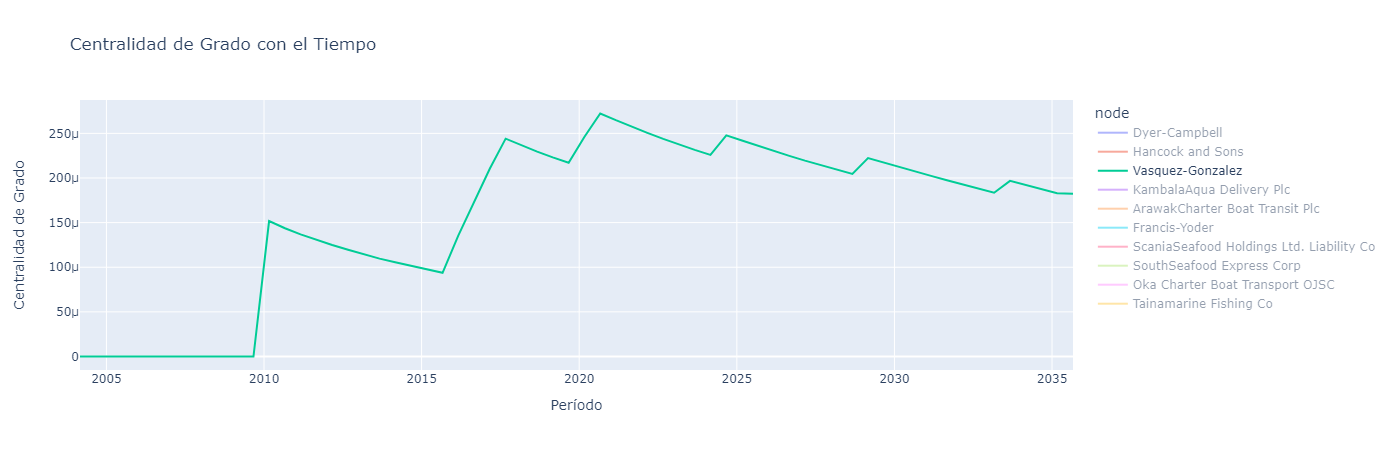
\includegraphics[width=0.7\linewidth]{graphs/grado_centralidad_tiempo_vasquez.png}
  \caption{Evolución de centralidad de grado para la empresa Vasquez-Gonzalez.}
  \label{fig:cent_grado_g_VG}
\end{figure}

\begin{figure}[H]
  \centering
  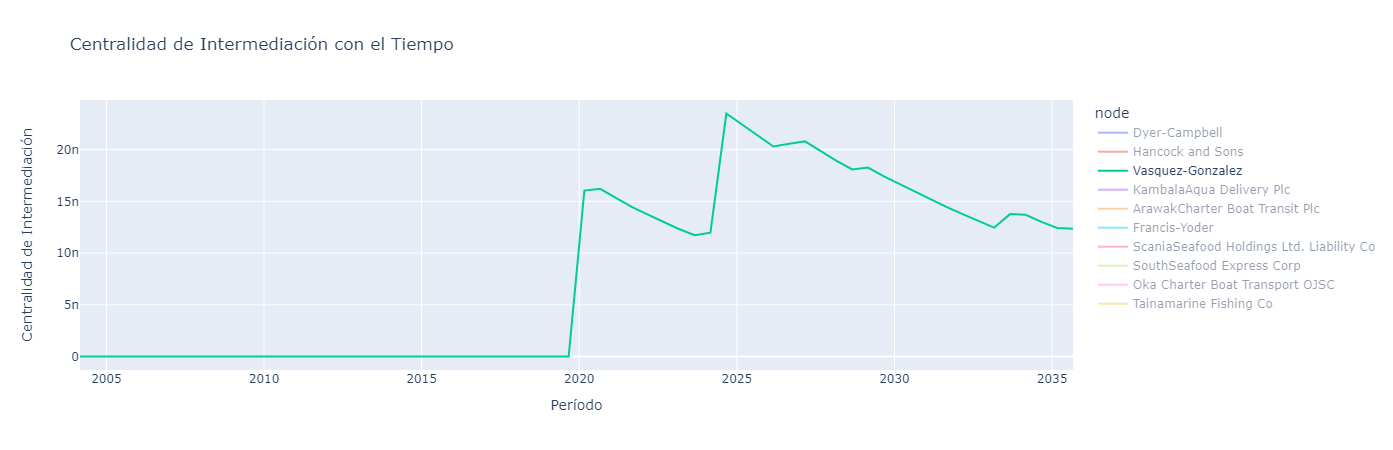
\includegraphics[width=0.7\linewidth]{graphs/between_centralidad_tiempo_vasquez.png}
  \caption{Evolución de centralidad de intermediación para la empresa Vasquez-Gonzalez.}
  \label{fig:cent_grado_i_VG}
\end{figure}

\paragraph{Inferencia de propiedad:}
Este segundo problema también se aborda mediante el análisis de los gráficos de evolución de centralidad. Se observa cómo los cambios en la centralidad pueden indicar cambios en la propiedad de las empresas a lo largo del tiempo, como se ilustra en el ejemplo mencionado anteriormente.

Este enfoque visual proporciona una comprensión profunda de cómo la evolución de la centralidad puede relacionarse tanto con la influencia como con la propiedad en el contexto empresarial a lo largo de períodos extensos.

\subsection{Análisis de cambios en la red después del incidente con SouthSeaFood}

En este estudio, analizamos los cambios en la estructura de la red después del incidente con SouthSeaFood. Observamos cómo las medidas de centralidad de las empresas afectadas cambiaron significativamente, destacando el ascenso de Polak como el nodo central de la red.

\section{Análisis de Centralidad}

Los gráficos de las figuras \ref{fig:cent_grado}, \ref{fig:cent_Betweenness} y \ref{fig:cent_autovector}, muestran las medidas de centralidad (grado, Betweenness y autovector) antes y después del incidente para cada empresa. Se observa que tanto el grado como el Betweenness disminuyeron considerablemente para todas las empresas después del incidente. Sin embargo, el autovector, aunque disminuyó para algunas empresas, aumentó sustancialmente para la empresa Polak, que no era prominente en este aspecto antes del incidente, pero ahora posee el mayor autovector entre todas las empresas.

\subsection{Centralidad de Grado}

\begin{figure}[H]
    \centering
    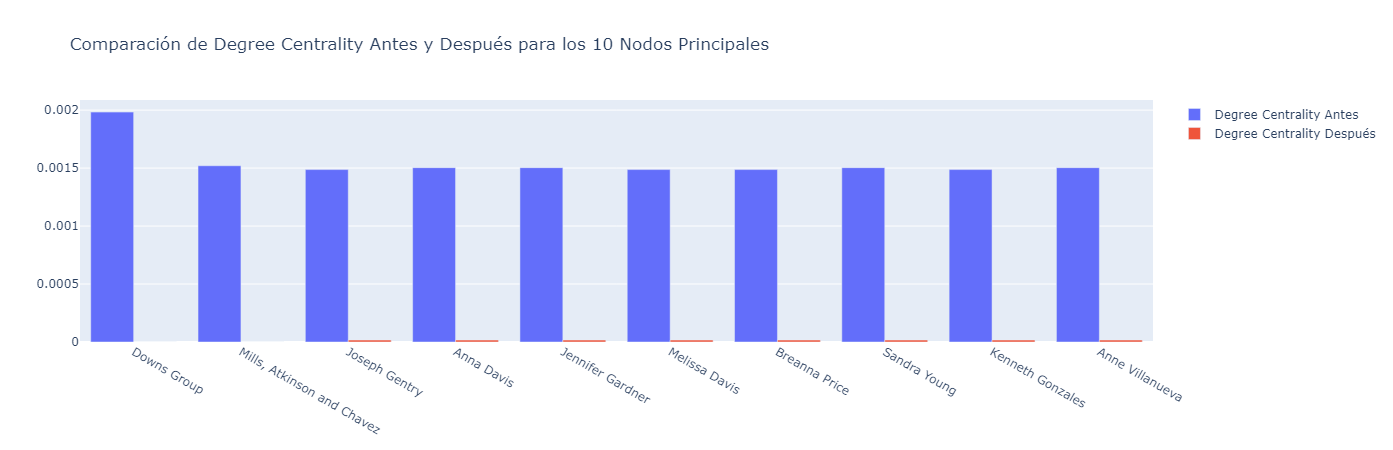
\includegraphics[width=0.8\linewidth]{graphs/degree_centrality_after_before_southseafood_top10.png}
    \caption{Centralidad de Grado antes y después del incidente con SouthSeaFood}
    \label{fig:cent_grado}
\end{figure}

\subsection{Centralidad de Betweenness}

\begin{figure}[H]
    \centering
    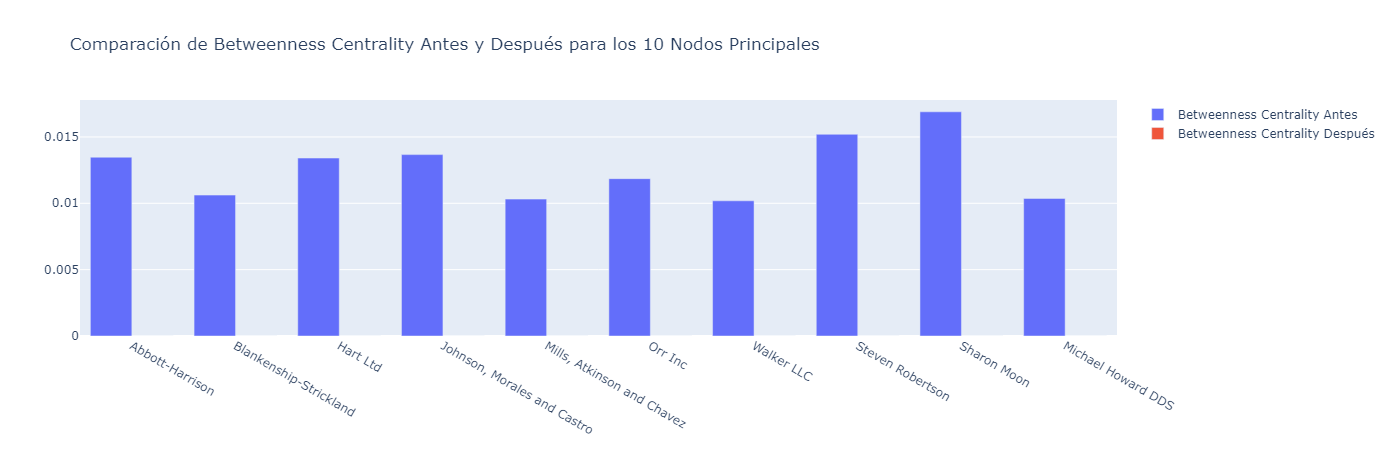
\includegraphics[width=0.8\linewidth]{graphs/betweeness_centrality_after_before_southseafood_top10.png}
    \caption{Centralidad de Betweenness antes y después del incidente con SouthSeaFood}
    \label{fig:cent_Betweenness}
\end{figure}

\subsection{Centralidad de autovector}

\begin{figure}[H]
    \centering
    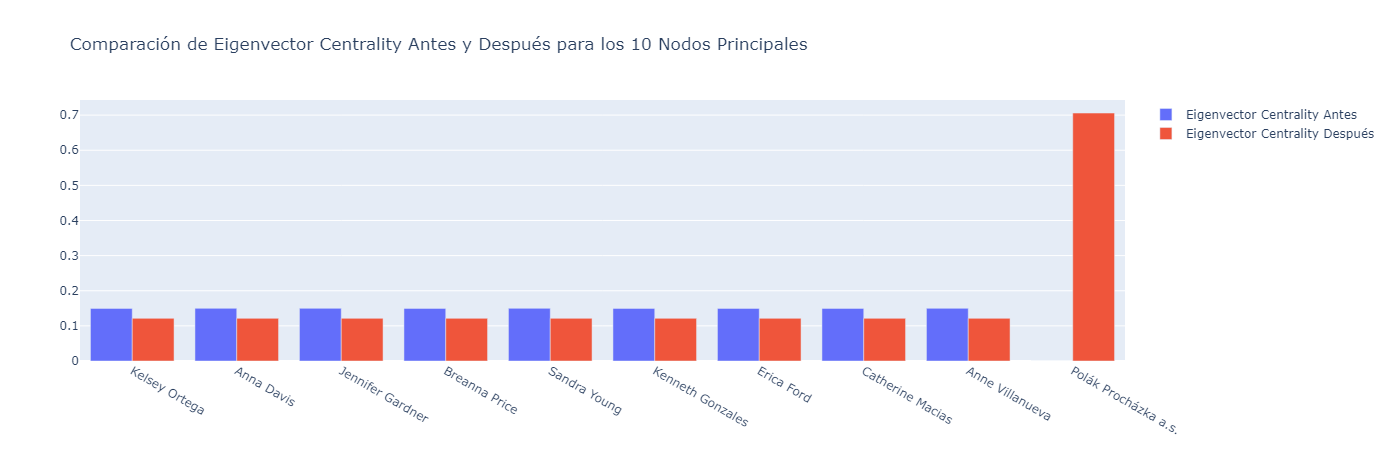
\includegraphics[width=0.8\linewidth]{graphs/eingenvector_centrality_after_before_southseafood_top10.png}
    \caption{Centralidad de autovector antes y después del incidente con SouthSeaFood}
    \label{fig:cent_autovector}
\end{figure}

El análisis de los cambios en las redes después del incidente con SouthSeaFood revela que la mayoría de las empresas que anteriormente tenían gran influencia perdieron esa posición. Notablemente, la empresa Polak emergió como el nuevo nodo central de la red, ya que su centralidad aumentó significativamente después del incidente.

% \section{Bibliografía}
\printbibliography[heading=bibintoc] % not numbered


\end{document}